\documentclass[11pt,letterpaper]{article}\usepackage[]{graphicx}\usepackage[]{color}
%% maxwidth is the original width if it is less than linewidth
%% otherwise use linewidth (to make sure the graphics do not exceed the margin)
\makeatletter
\def\maxwidth{ %
  \ifdim\Gin@nat@width>\linewidth
    \linewidth
  \else
    \Gin@nat@width
  \fi
}
\makeatother

\definecolor{fgcolor}{rgb}{0.345, 0.345, 0.345}
\newcommand{\hlnum}[1]{\textcolor[rgb]{0.686,0.059,0.569}{#1}}%
\newcommand{\hlstr}[1]{\textcolor[rgb]{0.192,0.494,0.8}{#1}}%
\newcommand{\hlcom}[1]{\textcolor[rgb]{0.678,0.584,0.686}{\textit{#1}}}%
\newcommand{\hlopt}[1]{\textcolor[rgb]{0,0,0}{#1}}%
\newcommand{\hlstd}[1]{\textcolor[rgb]{0.345,0.345,0.345}{#1}}%
\newcommand{\hlkwa}[1]{\textcolor[rgb]{0.161,0.373,0.58}{\textbf{#1}}}%
\newcommand{\hlkwb}[1]{\textcolor[rgb]{0.69,0.353,0.396}{#1}}%
\newcommand{\hlkwc}[1]{\textcolor[rgb]{0.333,0.667,0.333}{#1}}%
\newcommand{\hlkwd}[1]{\textcolor[rgb]{0.737,0.353,0.396}{\textbf{#1}}}%
\let\hlipl\hlkwb

\usepackage{framed}
\makeatletter
\newenvironment{kframe}{%
 \def\at@end@of@kframe{}%
 \ifinner\ifhmode%
  \def\at@end@of@kframe{\end{minipage}}%
  \begin{minipage}{\columnwidth}%
 \fi\fi%
 \def\FrameCommand##1{\hskip\@totalleftmargin \hskip-\fboxsep
 \colorbox{shadecolor}{##1}\hskip-\fboxsep
     % There is no \\@totalrightmargin, so:
     \hskip-\linewidth \hskip-\@totalleftmargin \hskip\columnwidth}%
 \MakeFramed {\advance\hsize-\width
   \@totalleftmargin\z@ \linewidth\hsize
   \@setminipage}}%
 {\par\unskip\endMakeFramed%
 \at@end@of@kframe}
\makeatother

\definecolor{shadecolor}{rgb}{.97, .97, .97}
\definecolor{messagecolor}{rgb}{0, 0, 0}
\definecolor{warningcolor}{rgb}{1, 0, 1}
\definecolor{errorcolor}{rgb}{1, 0, 0}
\newenvironment{knitrout}{}{} % an empty environment to be redefined in TeX

\usepackage{alltt}
\usepackage[letterpaper, margin = 1.0in]{geometry}
\usepackage[utf8]{inputenc}
\usepackage{amsmath}
\usepackage{amsfonts}
\usepackage{amssymb}
\usepackage{graphicx}
\usepackage{placeins}
\usepackage [english]{babel}
\usepackage [autostyle, english = american]{csquotes}
\MakeOuterQuote{"}
\usepackage{microtype}
\usepackage{setspace}% http://ctan.org/pkg/setspace
\AtBeginEnvironment{tabular}{\singlespacing}% Single spacing in tabular environment
\usepackage{booktabs}
\usepackage{titling}
\usepackage{fancyhdr}

\pagestyle{fancy}
\fancyhf{}
\rhead{\thepage}

\setlength{\droptitle}{-6em}   %Move title up 5
\renewcommand\maketitlehookb{\vspace{-3em}}  %Remove space after title
\renewcommand\maketitlehookc{\vspace{-2em}}  %Remove space after authors
\renewcommand\maketitlehookd{\vspace{-3em}}  %Remove space after date




%%%%%%%%%%%%%%%%%%%%%%%%%%%%%%%%%%%%%
%% DEFINING VARIABLES (START)
%%%%%%%%%%%%%%%%%%%%%%%%%%%%%%%%%%%%%
%% In this section, define the variables that change from semester to semester or
%% From user to user 
%%%%%%%%%%%%%%%%%%%%%%%%%%%%%%%%%%%%%

%% ----COURSE INFO---
\newcommand{\ClassNumber}{ME 274}		% Format ex: ME 274
\newcommand{\SemYear}{Spring 2018}		%Format ex: Spring 2018

%% ----REPORT HEADER INFO---
\author{Author Name1, Author Name2}
\title{\ClassNumber~Fundamentals Exam Summary Report: \SemYear \thanks{The source code that produced this report accompanied a journal manuscript that is in review.  For more details on how to prepare and interpret the results in this report, please watch for the journal article to be published.}} 
\lhead{\ClassNumber~FE Summary: \SemYear}

%% ---- INFO NEEDED FOR THE R CODE ---
%% ---- USERS SHOULD ONLY EDIT THE FOLLOWING CODE CHUNK!!! ---

%%%%%%%%%%%%%%%%%%%%%%%%%%%%%%%%%%%%%
%% DEFINING VARIABLES (END)
%%%%%%%%%%%%%%%%%%%%%%%%%%%%%%%%%%%%%


%%%%%%%%%%%%%%%%%%%%%%%%%%%%%%%%%%%%%
%% INSTRUCTOR REPORT (START)
%%%%%%%%%%%%%%%%%%%%%%%%%%%%%%%%%%%%%
\IfFileExists{upquote.sty}{\usepackage{upquote}}{}
\begin{document}
\maketitle




%%%%%%%%%%%%%%%%%%%%%%%%%%%%%%%%%
%% GRADE THE ASSESSMENT
%%%%%%%%%%%%%%%%%%%%%%%%%%%%%%%%%
% The code in the block below grade the responses from Gradescope and save some files in the working directory




%%%%%%%%%%%%%%%%%%%%%%%%%%%%%%%%%
%% CREATE AND SAVE THE ITEM RESPONSE CURVES FOR EACH QUESTION
%%%%%%%%%%%%%%%%%%%%%%%%%%%%%%%%%
% This section of the code creates the item response curves that are used in the instructor report






%%%%%%%%%%%%%%%%%%%%%%%%%%%%%%%%%
%% INSTRUCTOR SUMMARY REPORT
%%%%%%%%%%%%%%%%%%%%%%%%%%%%%%%%%
%This is where the actual content that is shown in the report starts.

\section*{Overall Performance}
Table \ref{table:summaryStats} lists the descriptive statistics for your students' total scores (the total number of questions correct). 
% latex table generated in R 3.3.2 by xtable 1.8-2 package
% Sat Jun 23 11:38:12 2018
\begin{table}[ht]
\centering
\caption{Summary Statistics for Overall Number of Questions Correct} 
\label{table:summaryStats}
\begin{tabular}{lcccccc}
  \toprule
 & Mean & Median & Minimum & Maximum & 1st Quartile & 3rd Quartile \\ 
  \midrule
All Sections & 8.36 & 8.00 & 6.00 & 11.00 & 7.00 & 9.50 \\ 
  Section 1 & 8.00 & 8.00 & 7.00 & 9.00 & 7.50 & 8.50 \\ 
  Section 2 & 8.00 & 8.00 & 6.00 & 10.00 & 7.00 & 9.00 \\ 
  Section 3 & 8.33 & 8.00 & 7.00 & 10.00 & 7.50 & 9.00 \\ 
  Section 4 & 9.00 & 9.00 & 7.00 & 11.00 & 8.00 & 10.00 \\ 
   \bottomrule
\end{tabular}
\end{table}

\FloatBarrier

\section*{Performance By Question}
Table \ref{table:questStats} details the proportion of correct responses for each question on the assessment.  

%\newpage

% latex table generated in R 3.3.2 by xtable 1.8-2 package
% Sat Jun 23 11:38:12 2018
\begin{table}[ht]
\centering
\caption{Proportion of Students That Answered Question Correctly} 
\label{table:questStats}
\begin{tabular}{lccccc}
  \toprule 
 & \multicolumn{5}{c}{Section}\\
 \cline{2-6} 
 & All & 1 & 2 & 3 & 4 \\ 
  \midrule 
Q3. Cross Product: Conceptual & 0.91 & 1.00 & 0.67 & 1.00 & 1.00 \\ 
  Q10. Vector Projection: Coord. System & 0.91 & 1.00 & 0.67 & 1.00 & 1.00 \\ 
  Q1. Speed Time History & 0.82 & 0.50 & 1.00 & 1.00 & 0.67 \\ 
  Q4. Free Body Diagrams & 0.82 & 0.50 & 0.67 & 1.00 & 1.00 \\ 
  Q7. Cross Product: Calculation & 0.82 & 1.00 & 0.67 & 0.67 & 1.00 \\ 
  Q11. Vector Projection: Rotated Coord. System & 0.82 & 1.00 & 0.67 & 0.67 & 1.00 \\ 
  Q8. Friction & 0.73 & 0.50 & 0.67 & 1.00 & 0.67 \\ 
  Q6. Vector Projection: Unit Vector & 0.64 & 1.00 & 0.67 & 0.33 & 0.67 \\ 
  Q12. Moments & 0.64 & 1.00 & 0.67 & 0.33 & 0.67 \\ 
  Q2. Kinetic Energy Time History & 0.55 & 0.00 & 1.00 & 0.67 & 0.33 \\ 
  Q9. FBD and Multibody Systems & 0.55 & 0.00 & 0.67 & 0.67 & 0.67 \\ 
  Q5. Chain Rule & 0.18 & 0.50 & 0.00 & 0.00 & 0.33 \\ 
   \bottomrule 
\end{tabular}
\end{table}


\newpage

\section*{How Did Your Students Answer the Questions?}
This section details how your students answered each of the questions.  The ``item response curves'' (IRCs) show how students with different overall test scores answered the questions.  

\subsection*{How to Read the IRC Plots}

\subsubsection*{Top Plot: Histogram of Total Scores}
The top plot is a histogram of the students' total test scores. It is repeated above every IRC for easy reference.  The information in the IRC is most reliable for the total test scores that students earned most frequently because the information is averaged over many students.  Thus, the information in the IRCs for the extreme scores is less reliable than the information near the median score.

\subsubsection*{Bottom Plot: IRCs}
The IRC plots should be read vertically for each total score.  In other words, for a given total test score, instructors should read vertically to see what proportion of students with that score selected a given answer choice.

However, the pattern of the proportion of a given answer option across total test scores can also be insightful.  
\begin{itemize}
	\item Ideally, the correct answer should draw an `s-shaped' curve when viewing the responses from lowest to highest total score.  This s-shaped curve indicates that the item clearly discriminates between those who understand the concept and those who do not, and it also likely reflects the validity and clarity of the question.
	\item IRCs for incorrect answers that look like inverted s-curves (higher for low scores and curving down to no responses for high scores) indicate high-functioning distractors.  These answers probably correspond to common misconceptions about the topic being assessed.
	\item Answer options that were chosen infrequently across all total test scores are low-functioning distractors because students do not consider them viable answers. You may want to revise or replace these answer choices.
\end{itemize}

\noindent \underline{Example:}  Suppose answer "C" was a popular choice for lower-performing students, and answer "B" (the correct answer) was popular with higher-performing students.  This scenario may imply that answer "C" is a common misconception that the instructor may want to address in class.

\subsubsection*{Summary and More Information} 
In summary, instructors can quickly look at the IRC patterns of: (i) lower-performing students to better understand what misconceptions the students may be harboring, and (ii) higher-performing students for evidence of question validity.  \\

\noindent More information can be found in the following references:
\begin{footnotesize}
	\begin{itemize}
	  \item Morris, G. A., Harshman, N., Branum-Martin, L., Mazur, E., Mzoughi, T., \& Baker, S. D. (2012). An item response curves analysis of the Force Concept Inventory. \textit{American Journal of Physics, 80}(9), 825-831. doi:10.1119/1.4731618
	  \item Morris, G. A., Branum-Martin, L., Harshman, N., Baker, S. D., Mazur, E., Dutta, S., . . . McCauley, V. (2006). Testing the test: Item response curves and test quality. \textit{American Journal of Physics, 74}(5), 449-453. doi:10.1119/1.2174053
	\end{itemize}
\end{footnotesize}

%%%%%%%%%%%%%%%%%%%%%%%%%%%%%%%%%
%% Insert the IRC plots to the instructor report
%%%%%%%%%%%%%%%%%%%%%%%%%%%%%%%%%
%This section loops through all the IRC plots and inserts them into the instructor report
\subsection*{Q1. Speed Time History}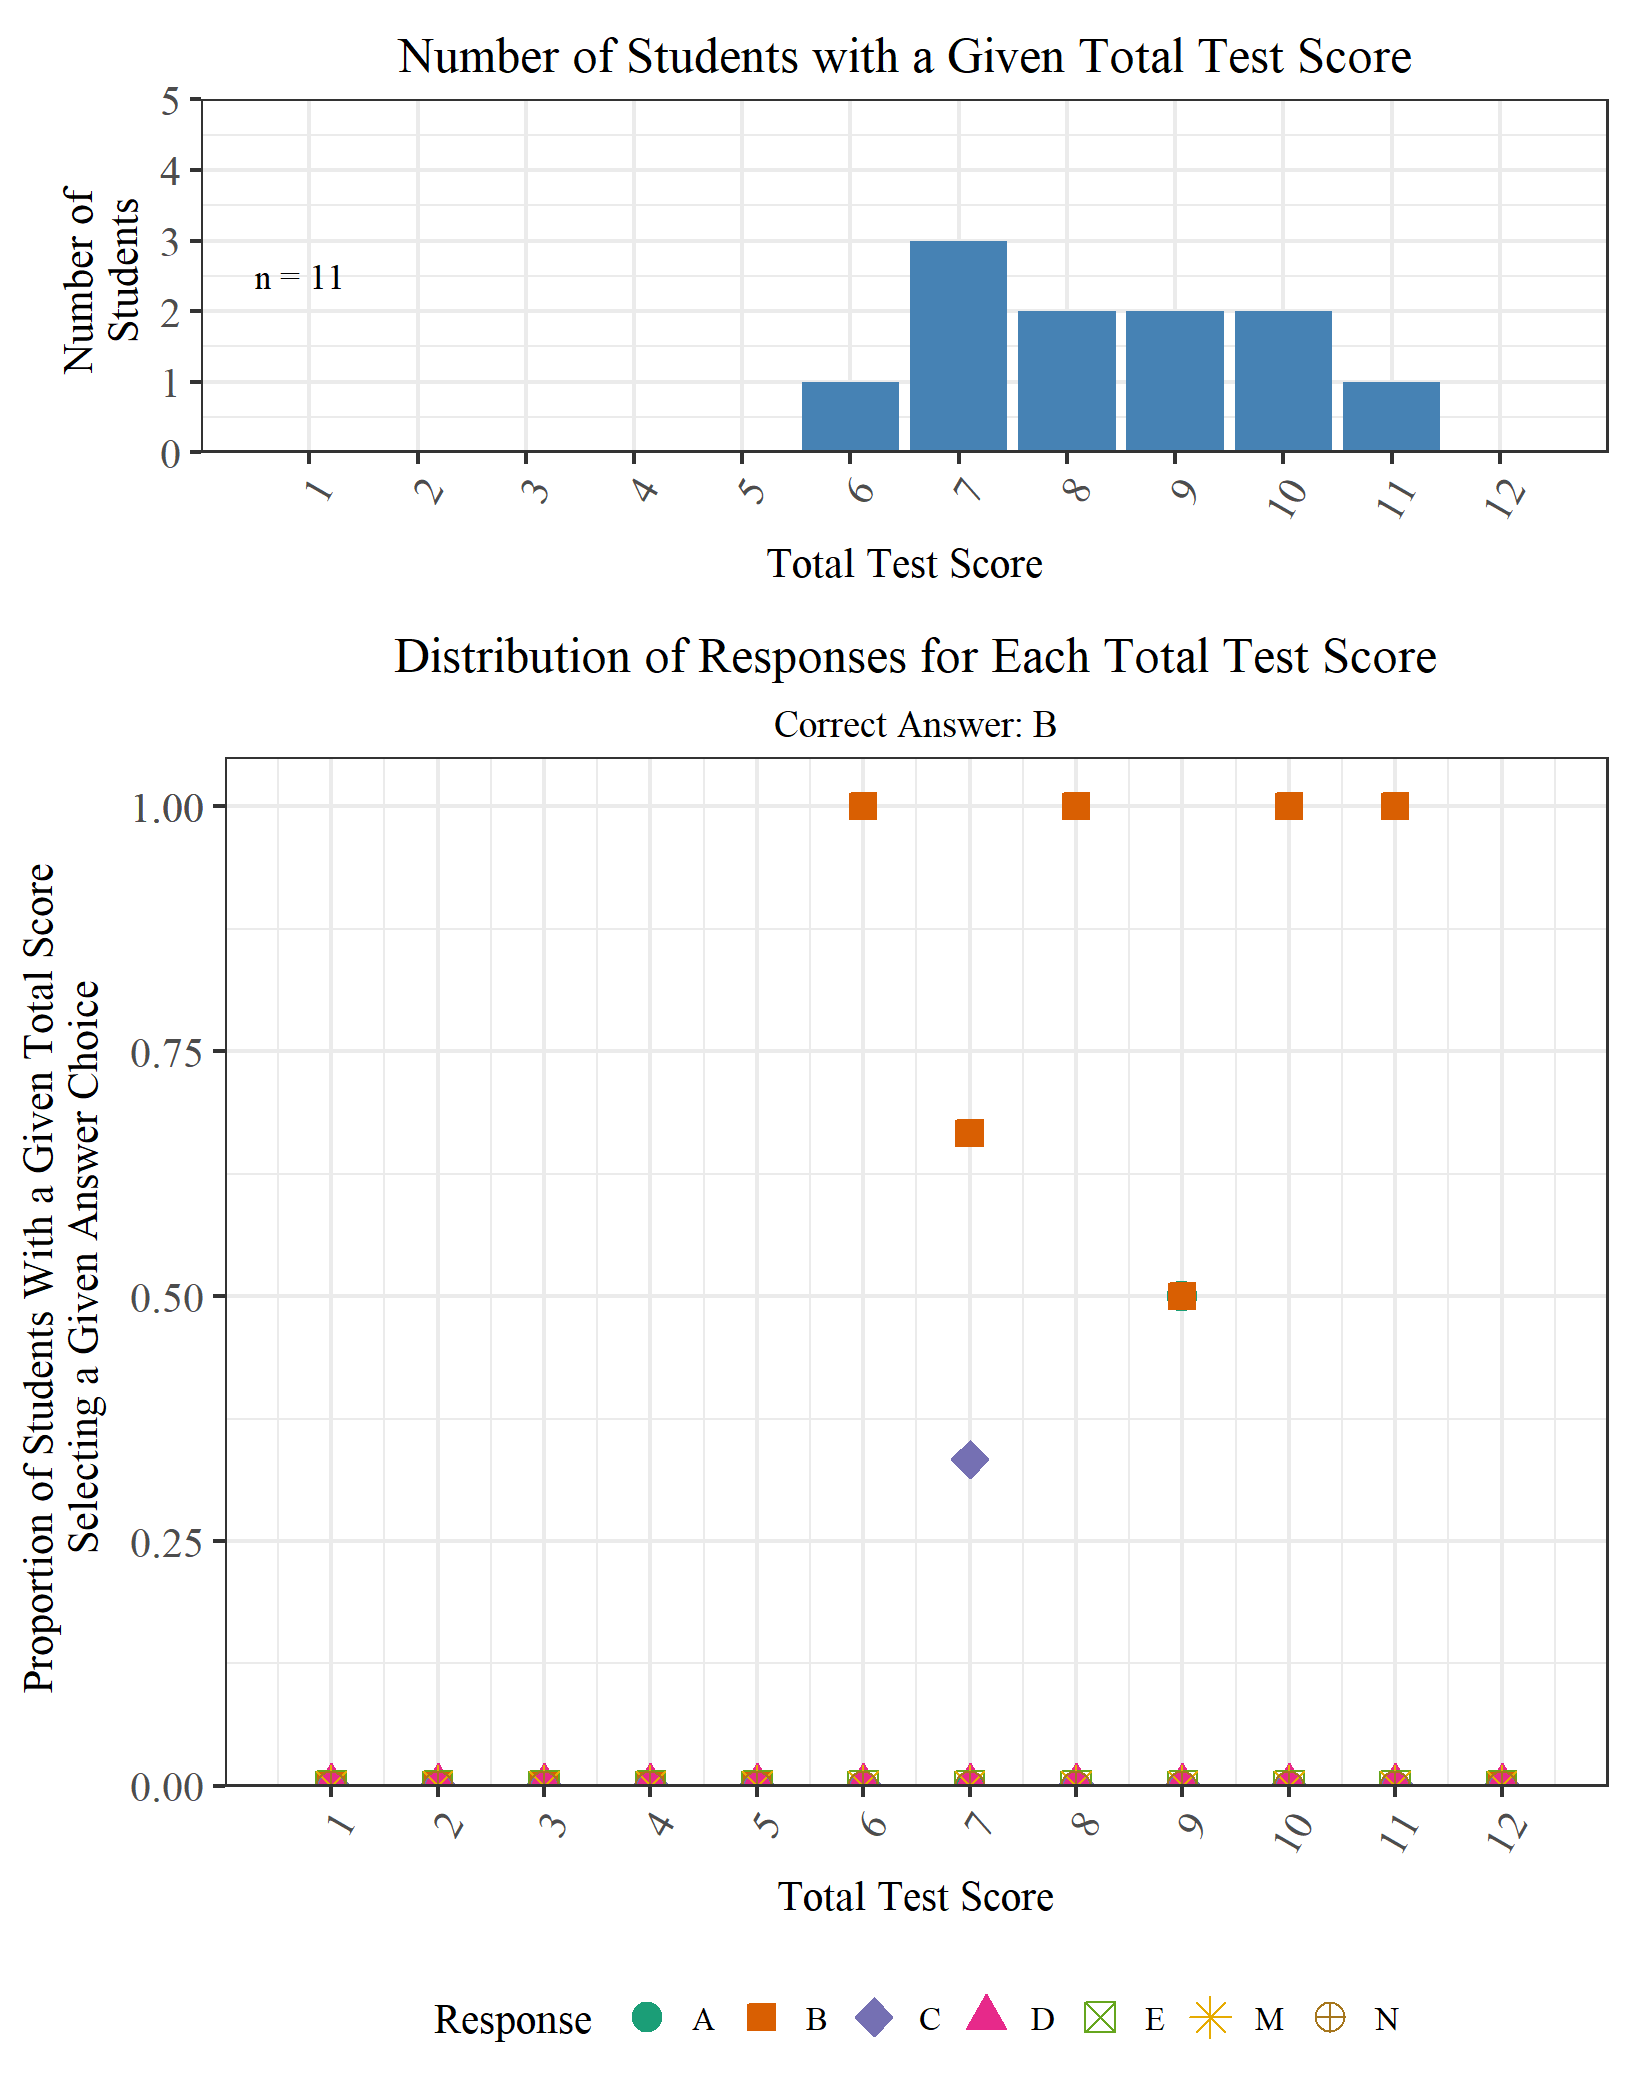
\includegraphics[width=\maxwidth]{IRC_1.png}\newpage\subsection*{Q2. Kinetic Energy Time History}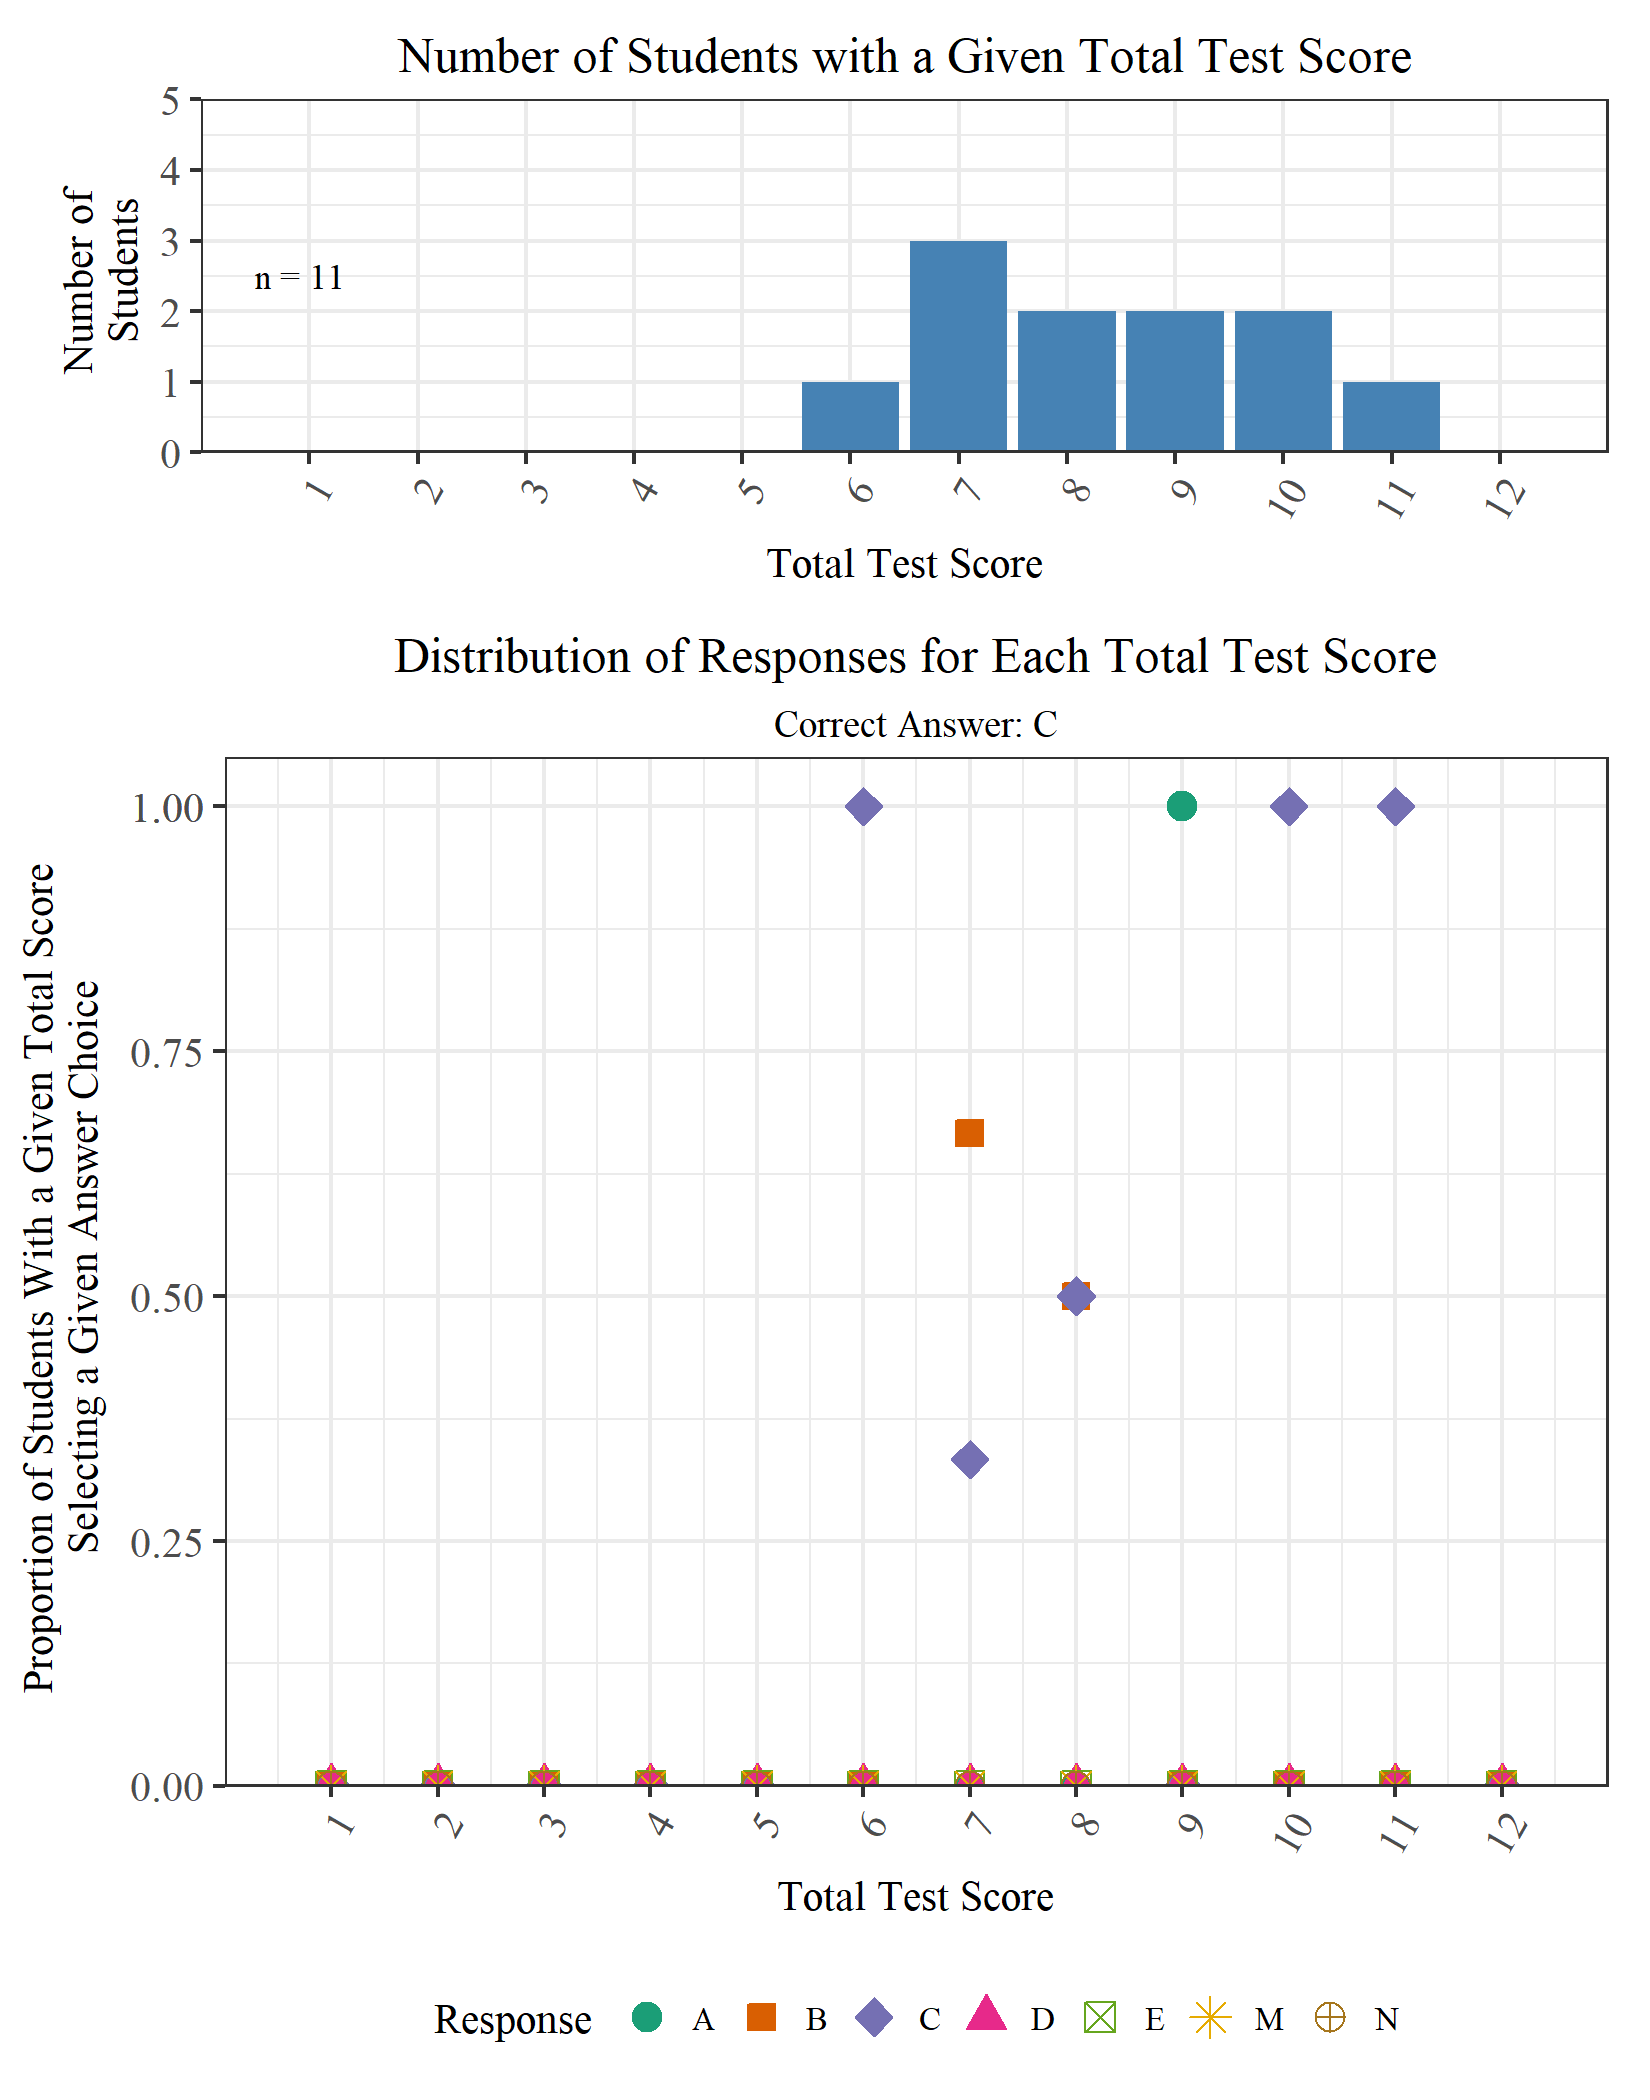
\includegraphics[width=\maxwidth]{IRC_2.png}\newpage\subsection*{Q3. Cross Product: Conceptual}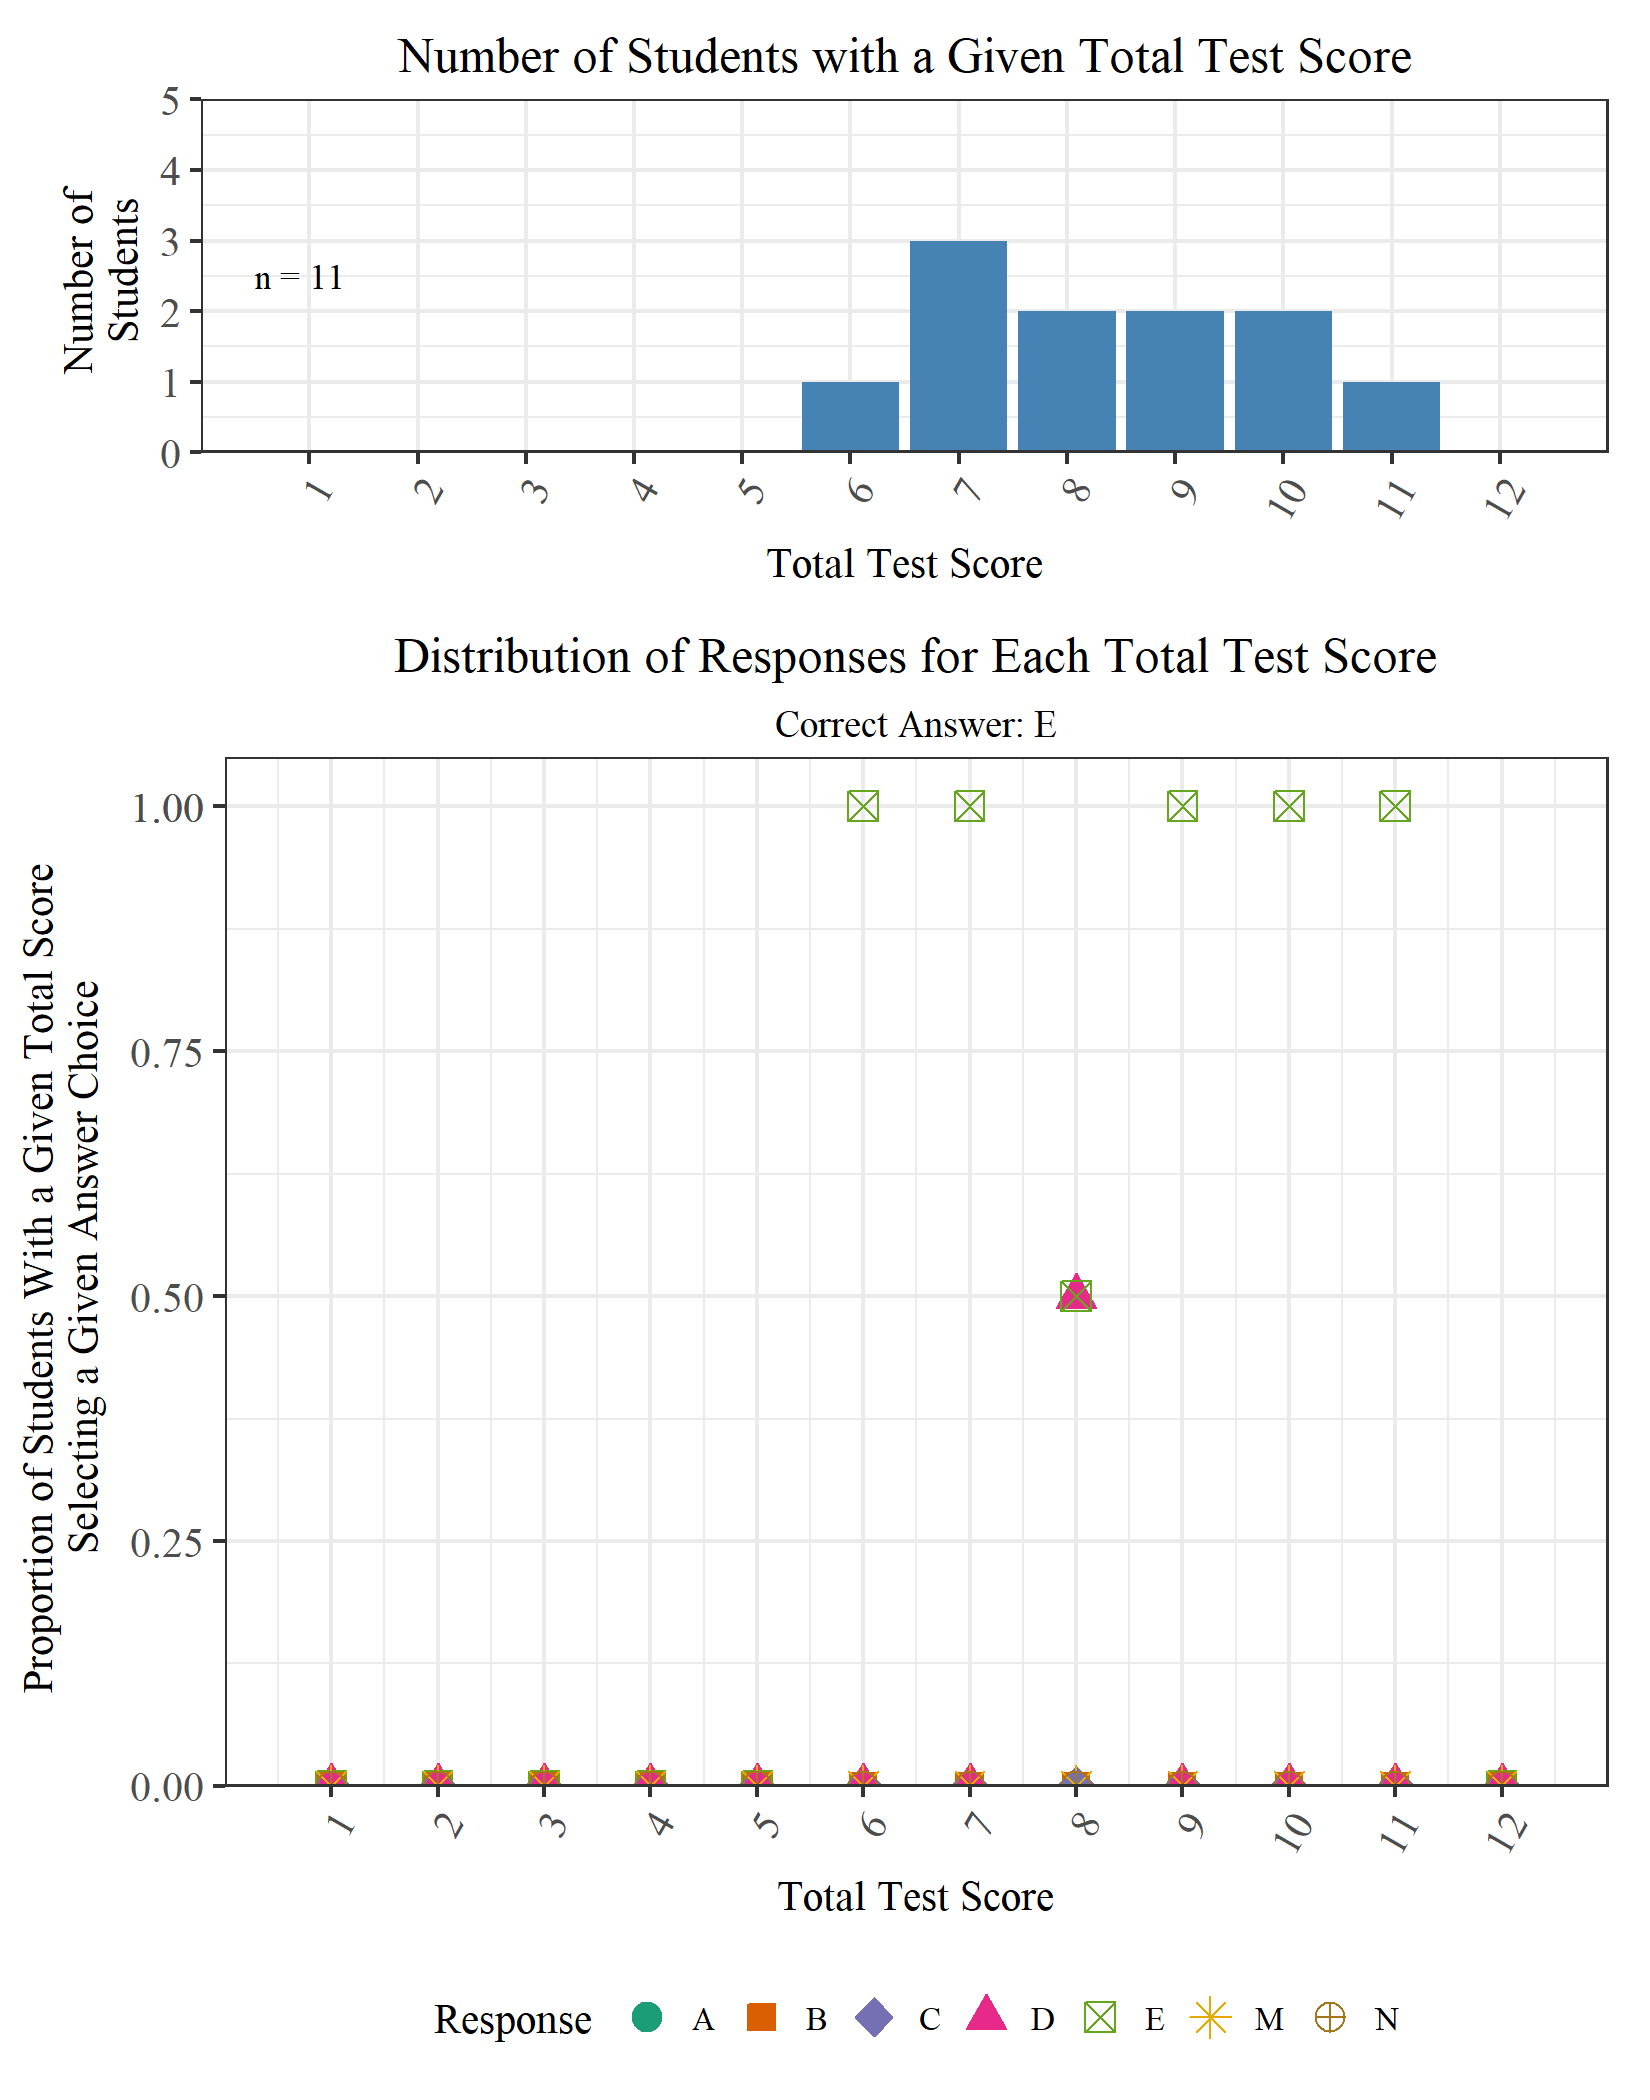
\includegraphics[width=\maxwidth]{IRC_3.png}\newpage\subsection*{Q4. Free Body Diagrams}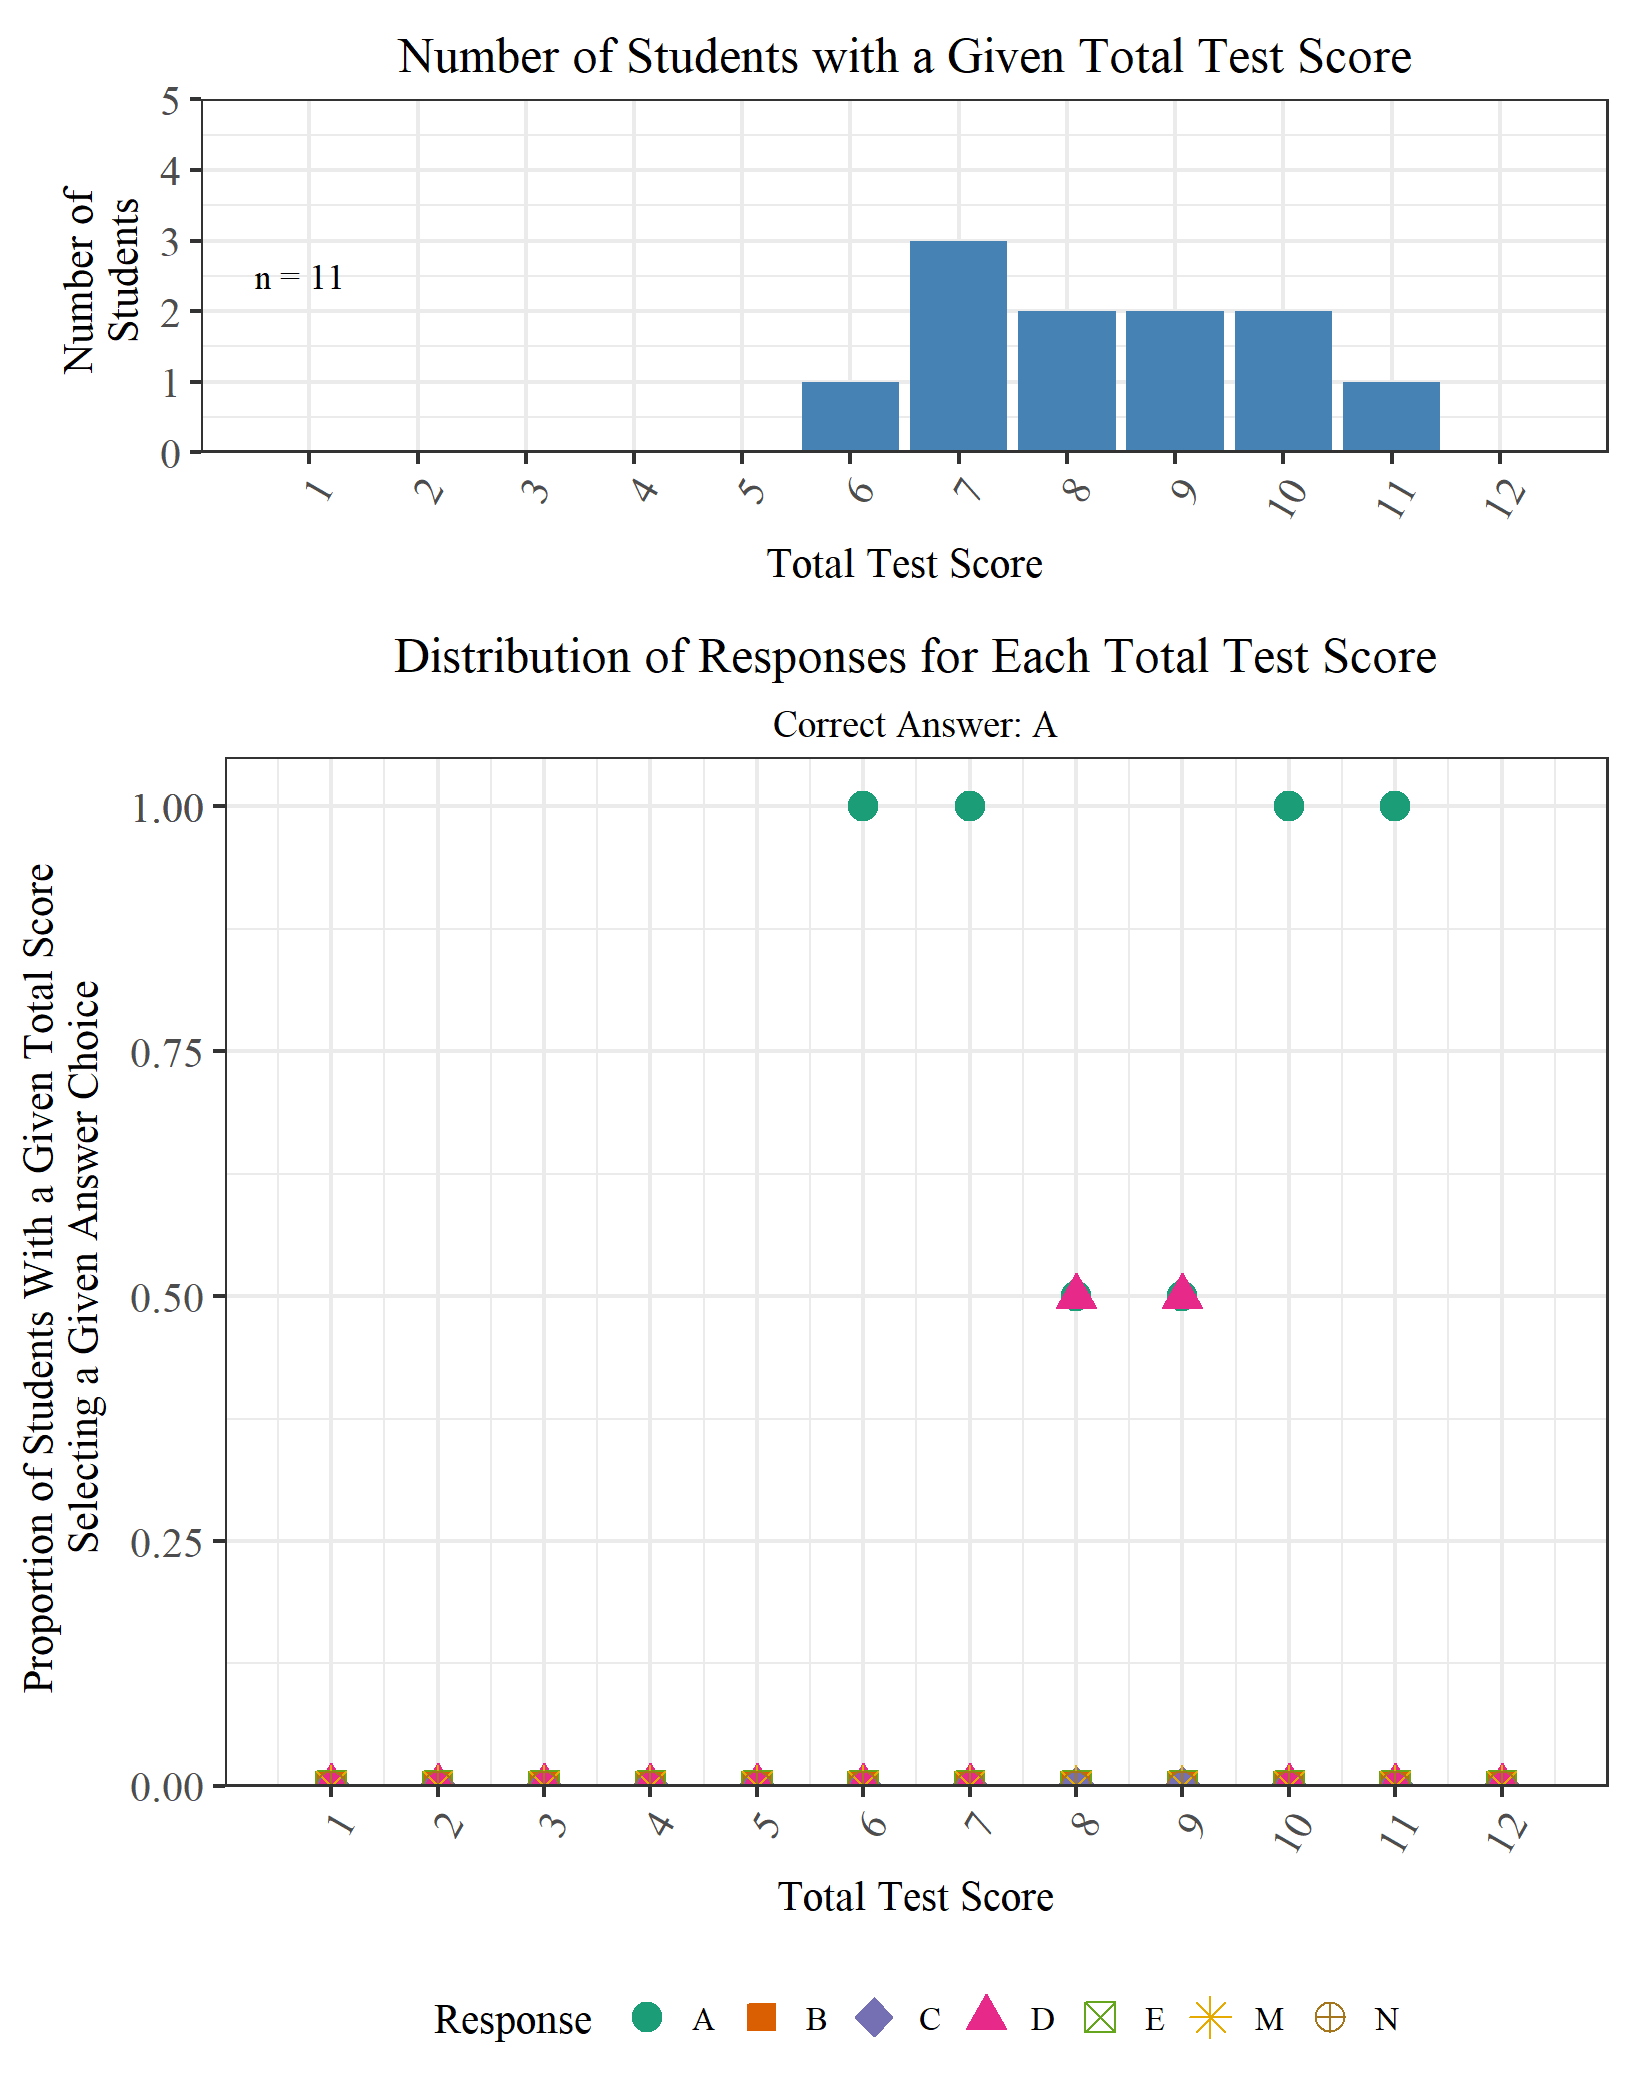
\includegraphics[width=\maxwidth]{IRC_4.png}\newpage\subsection*{Q5. Chain Rule}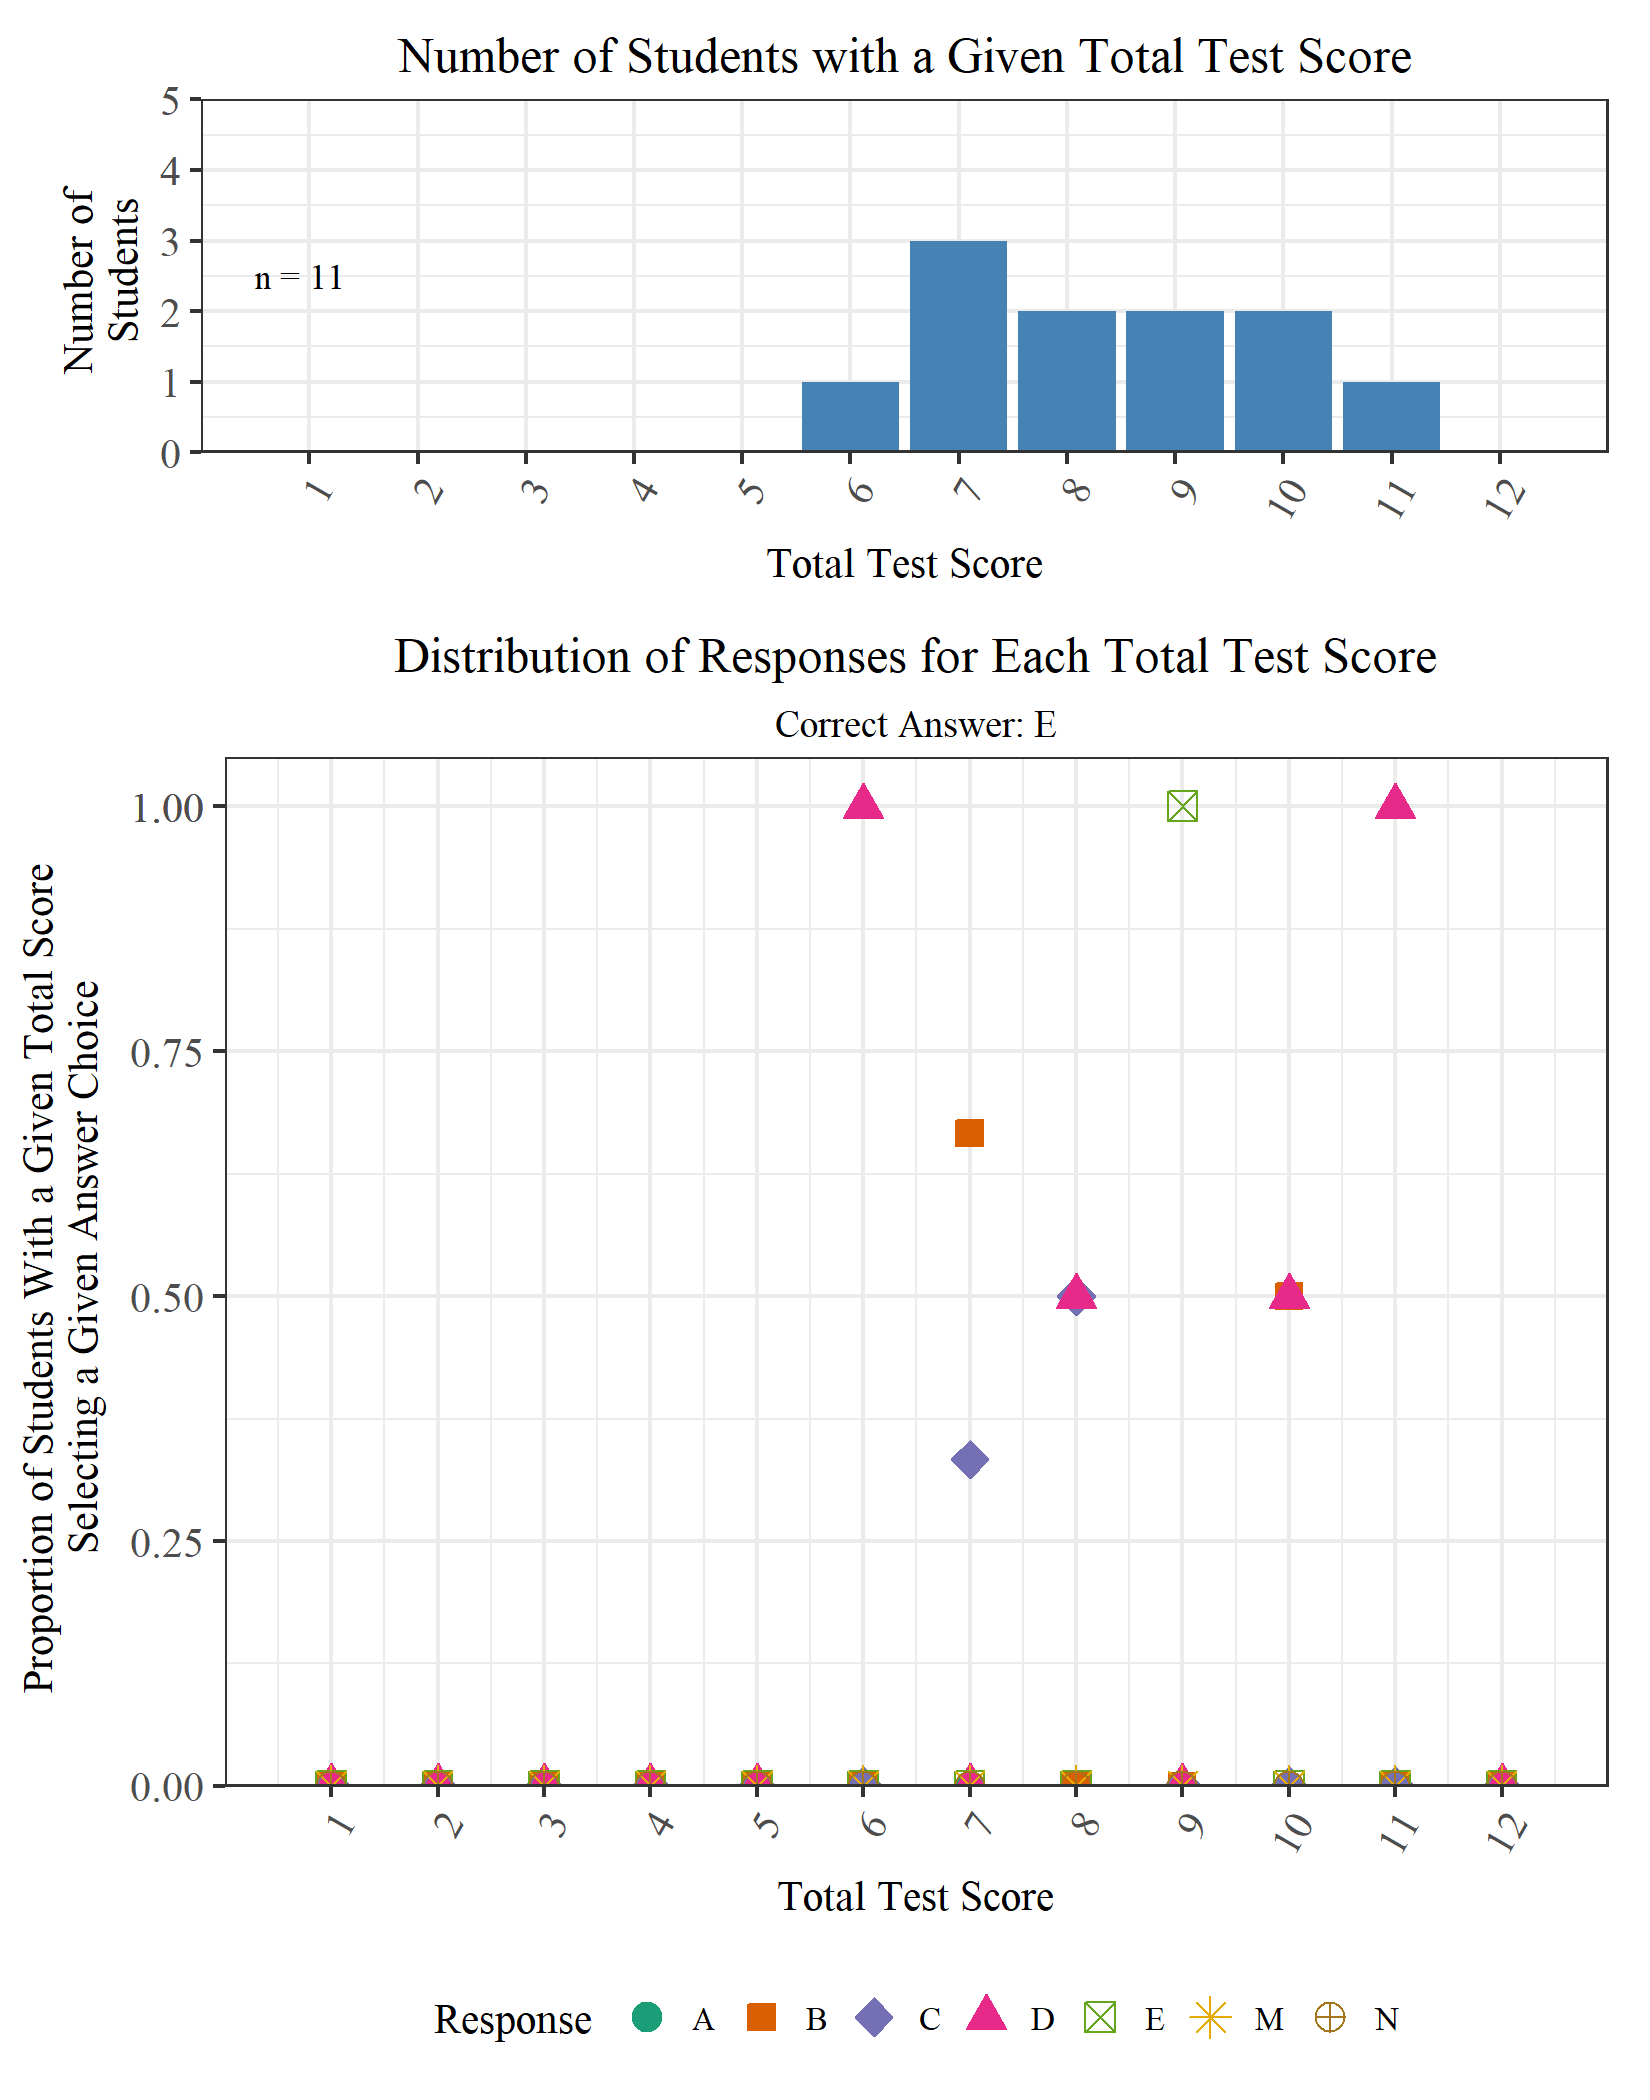
\includegraphics[width=\maxwidth]{IRC_5.png}\newpage\subsection*{Q6. Vector Projection: Unit Vector}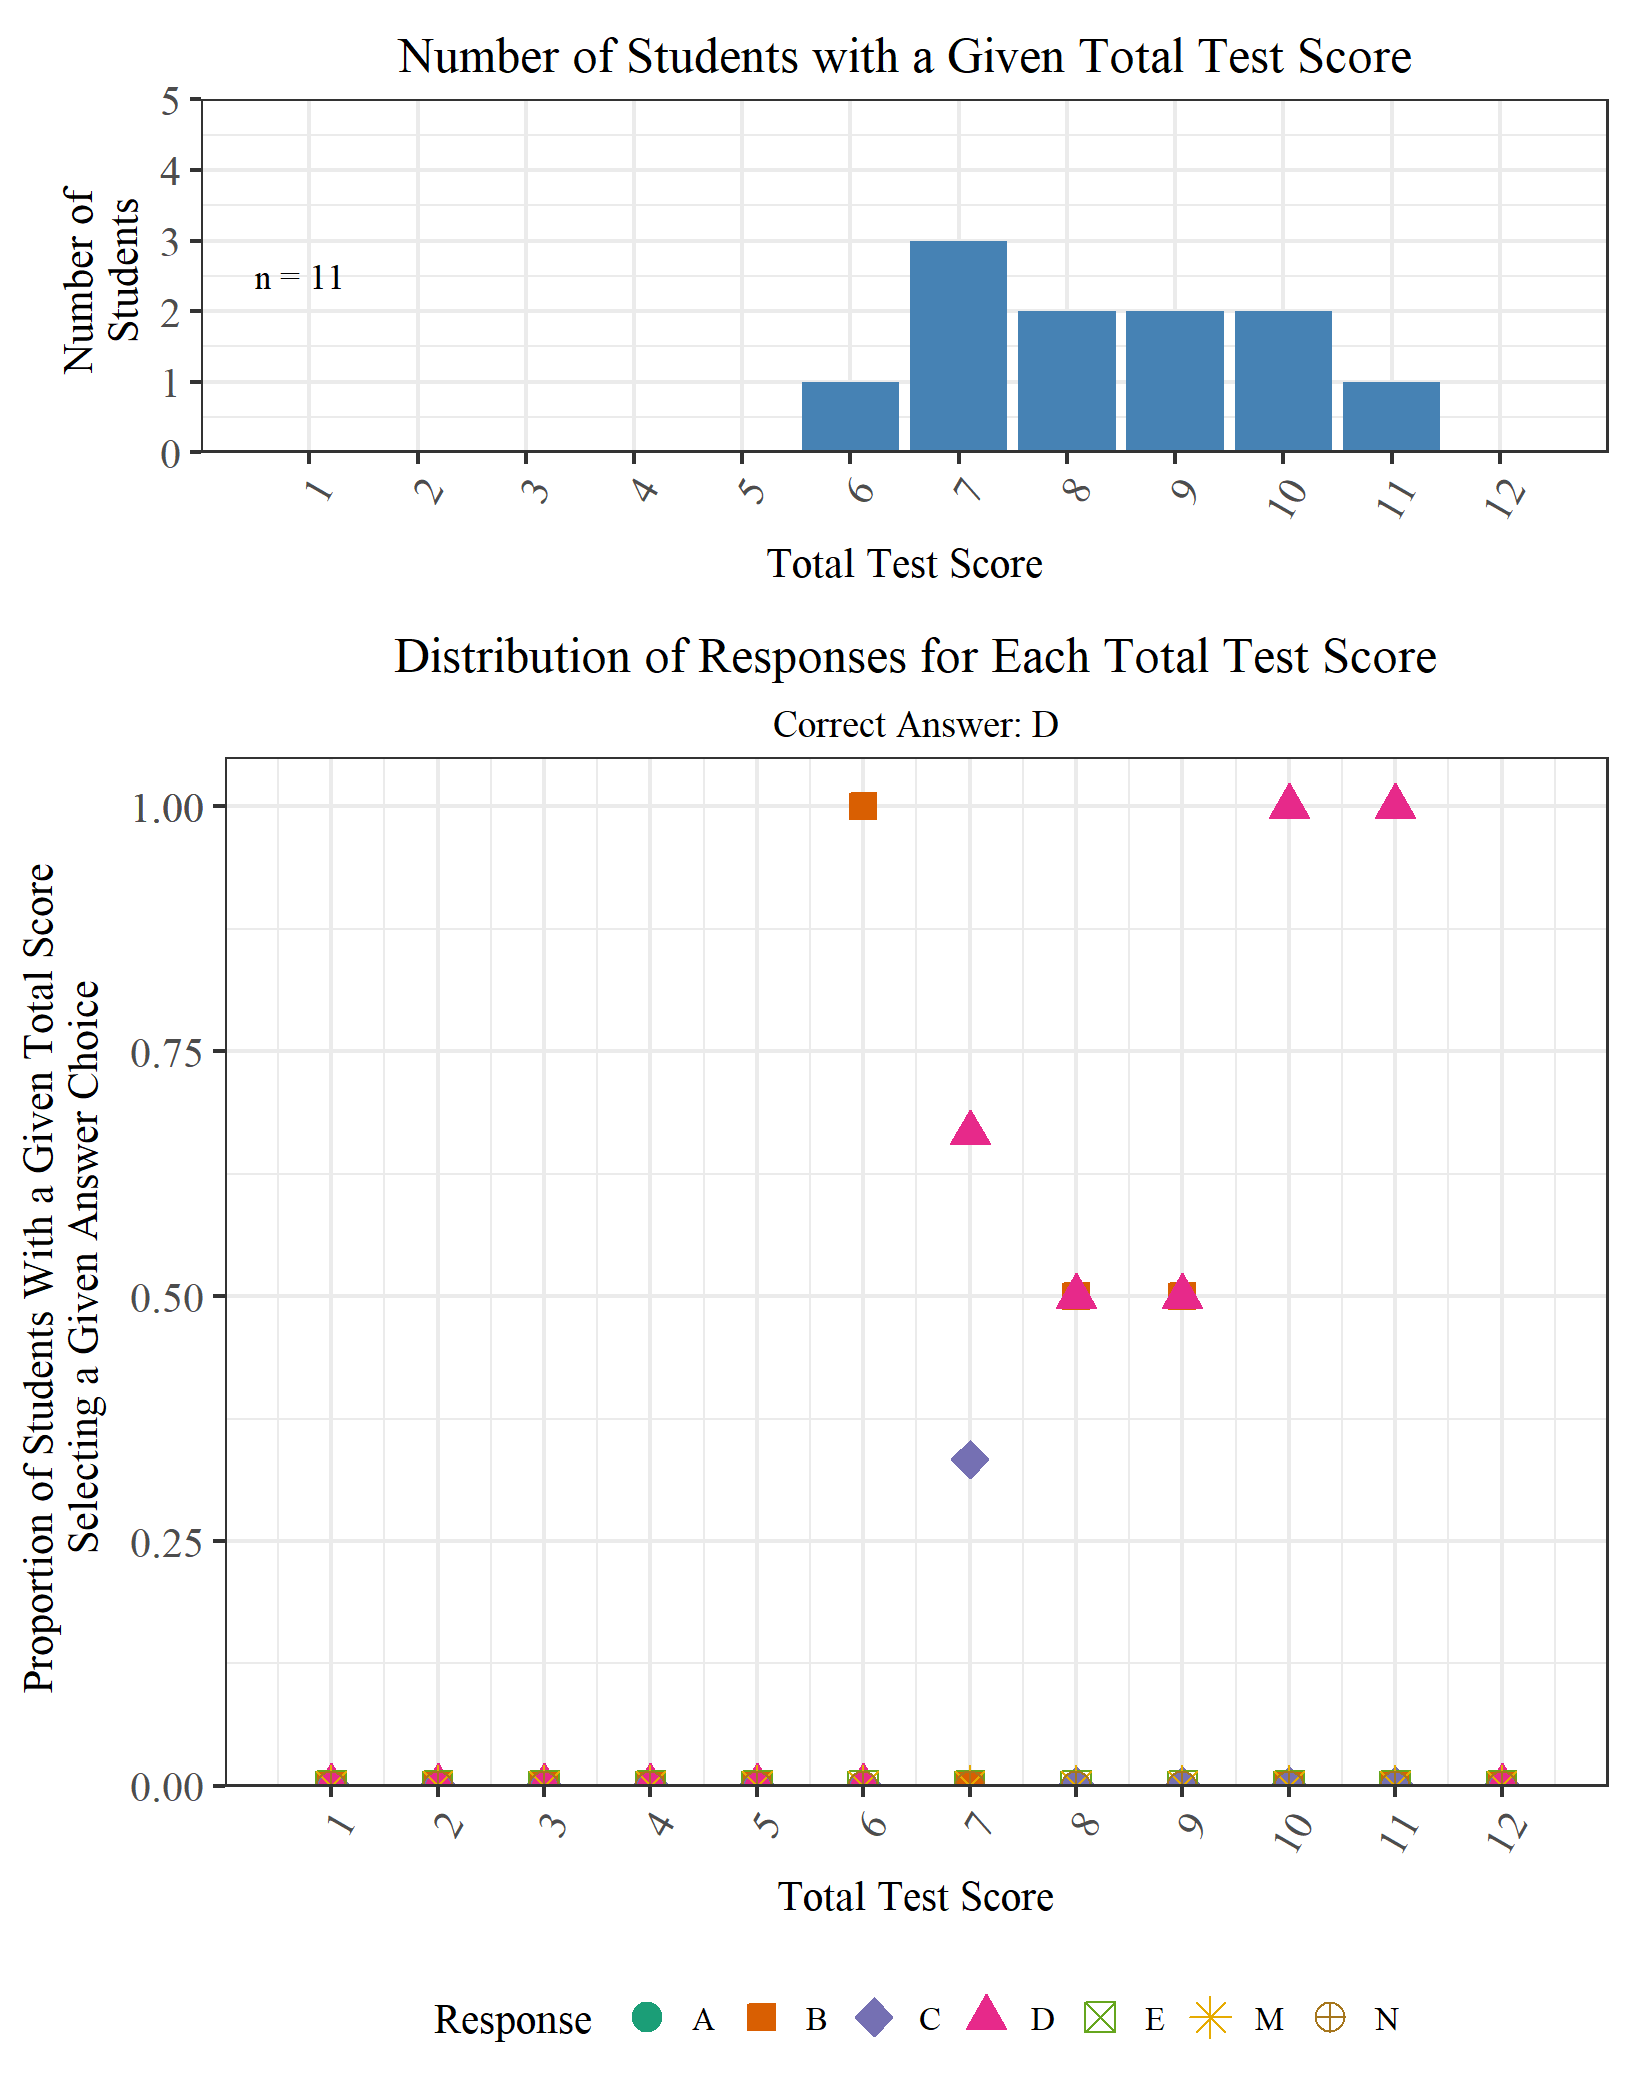
\includegraphics[width=\maxwidth]{IRC_6.png}\newpage\subsection*{Q7. Cross Product: Calculation}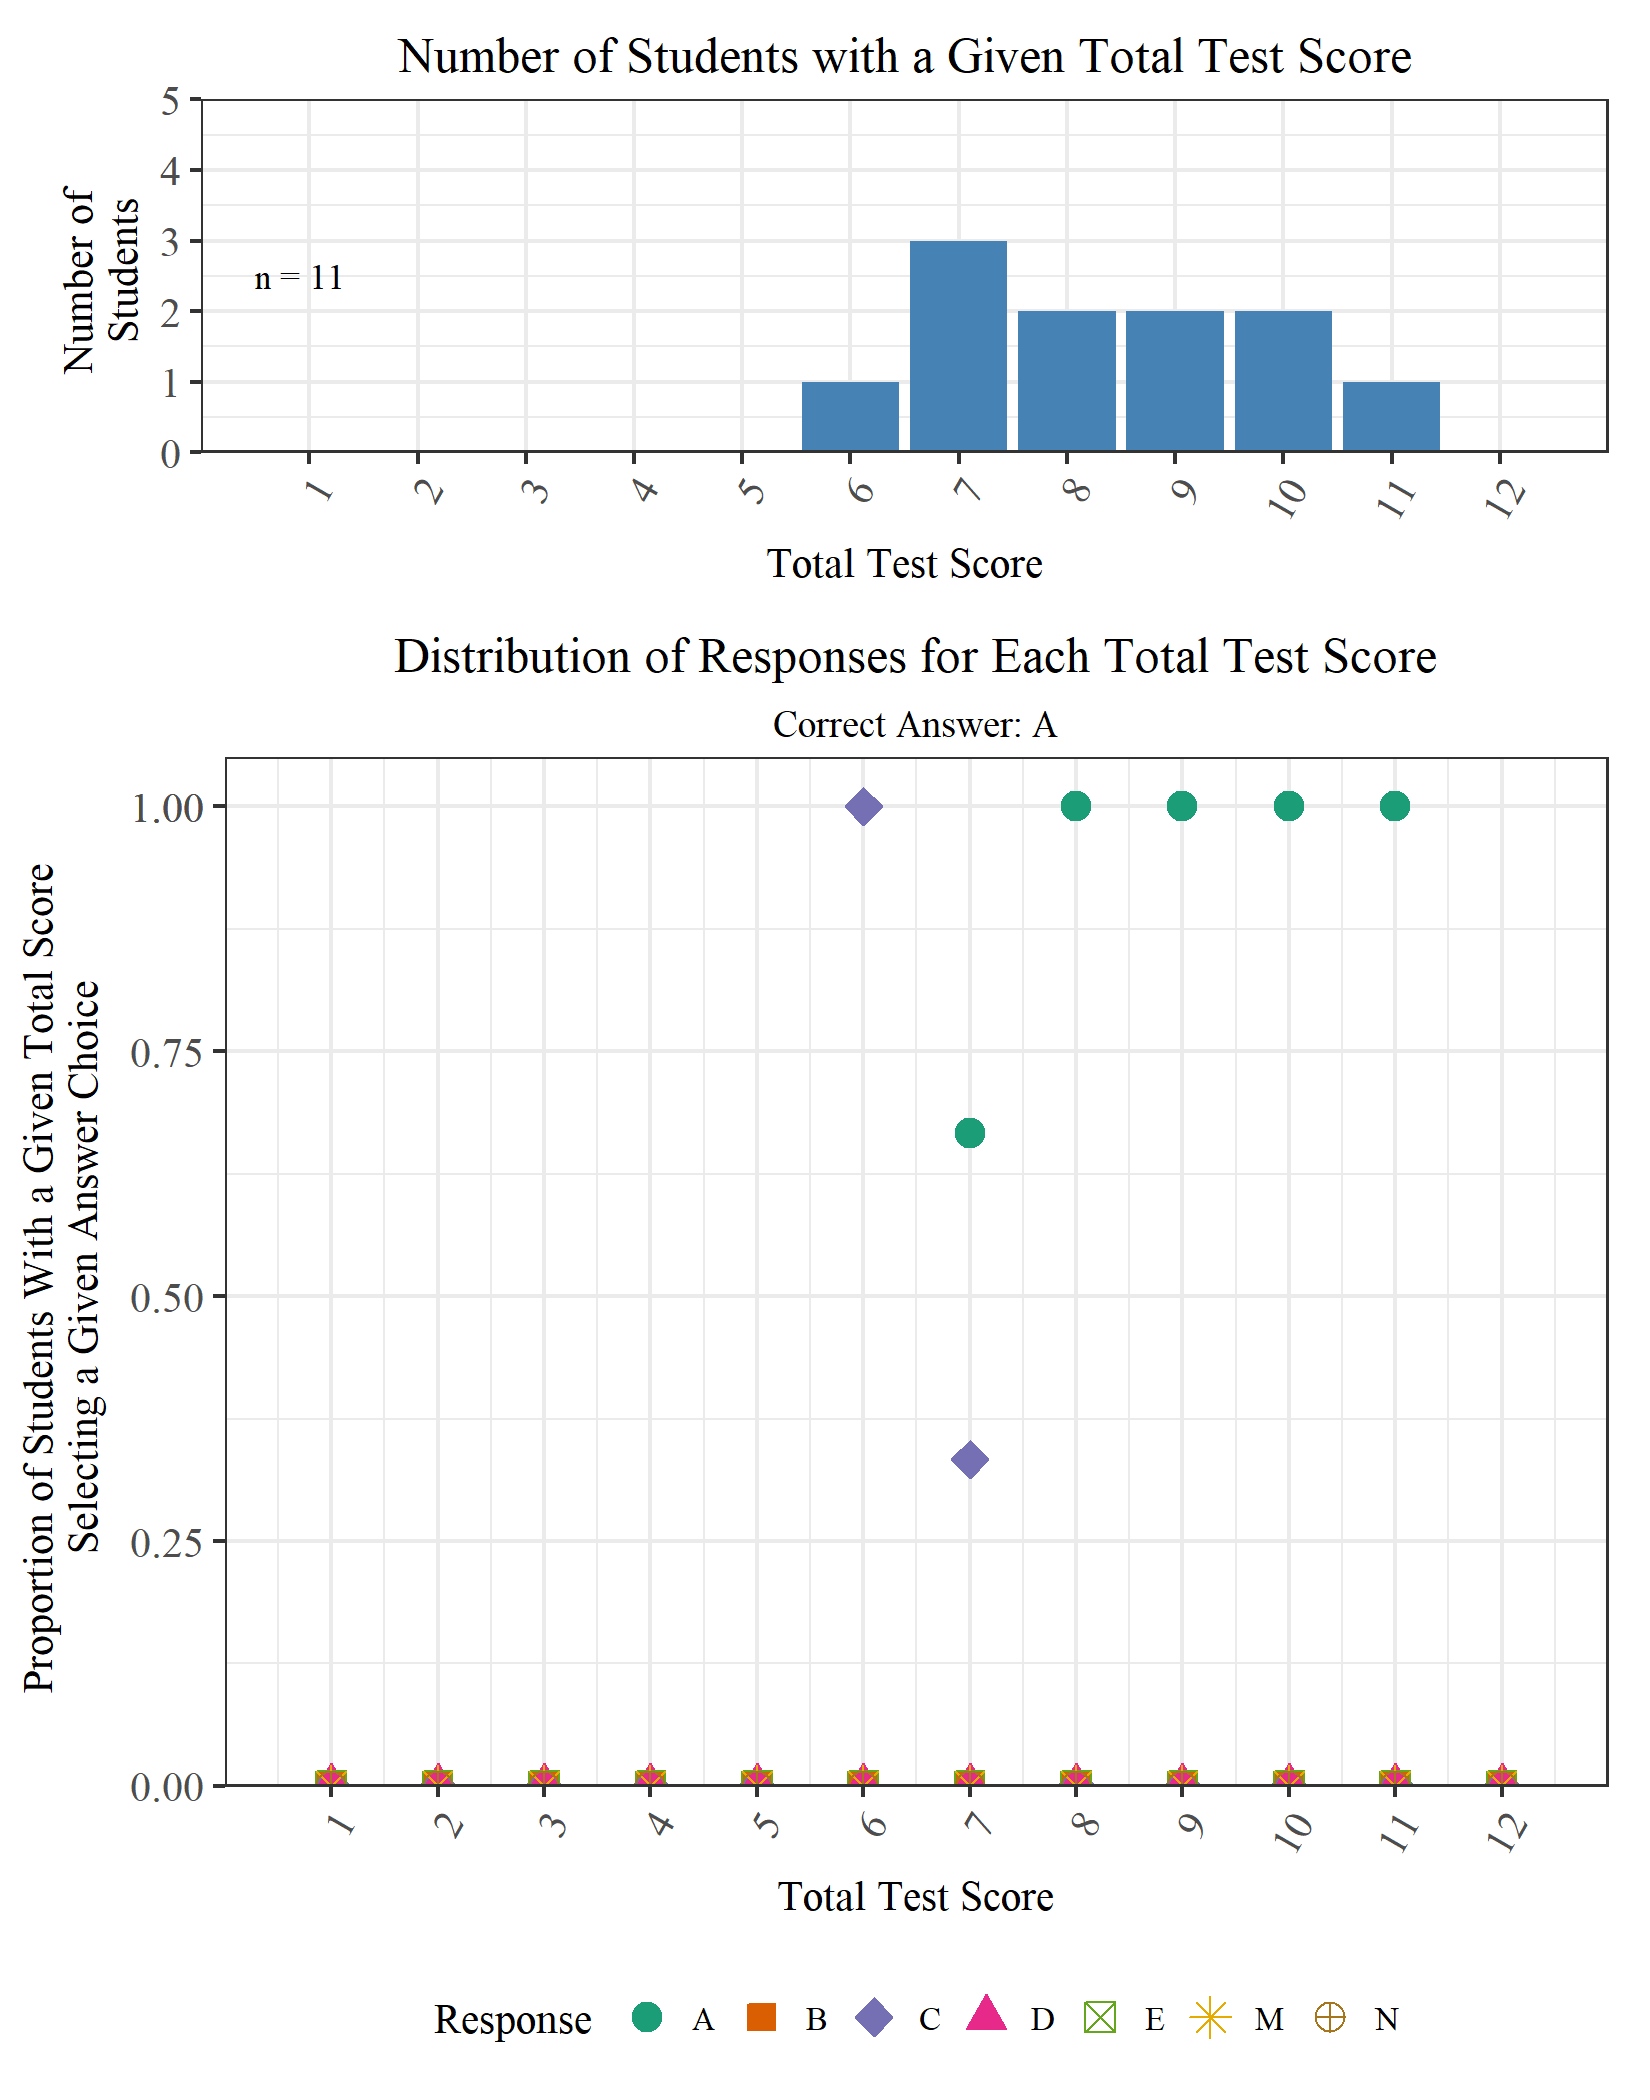
\includegraphics[width=\maxwidth]{IRC_7.png}\newpage\subsection*{Q8. Friction}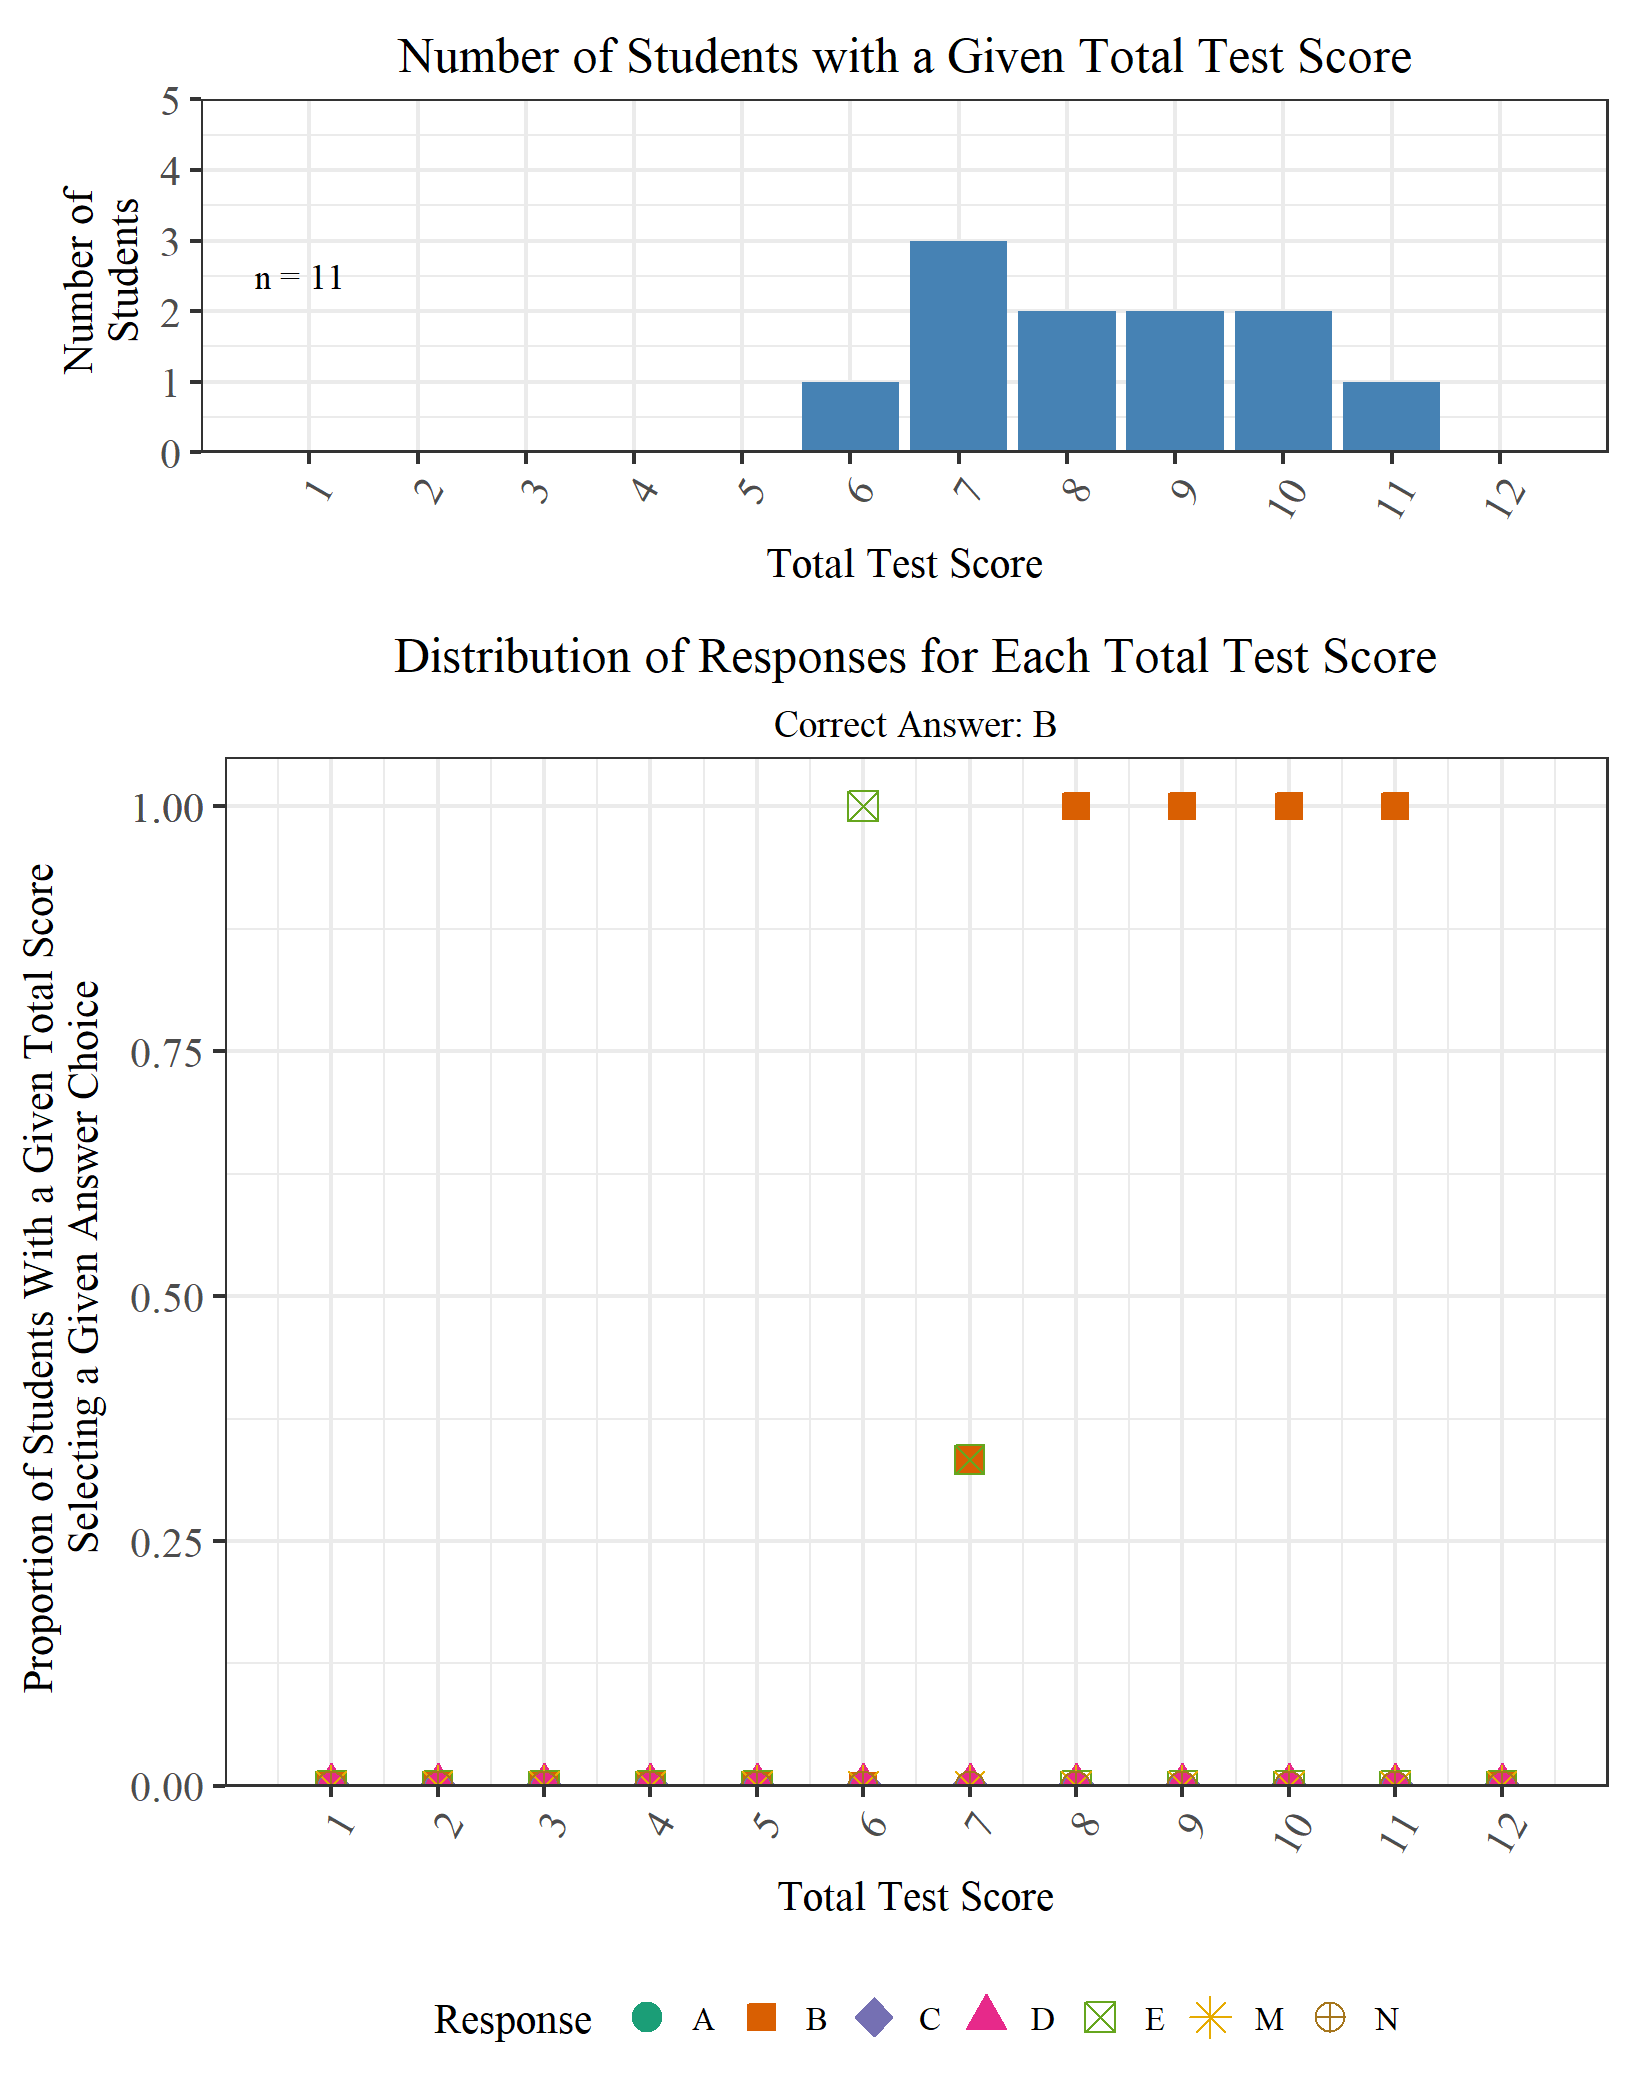
\includegraphics[width=\maxwidth]{IRC_8.png}\newpage\subsection*{Q9. FBD and Multibody Systems}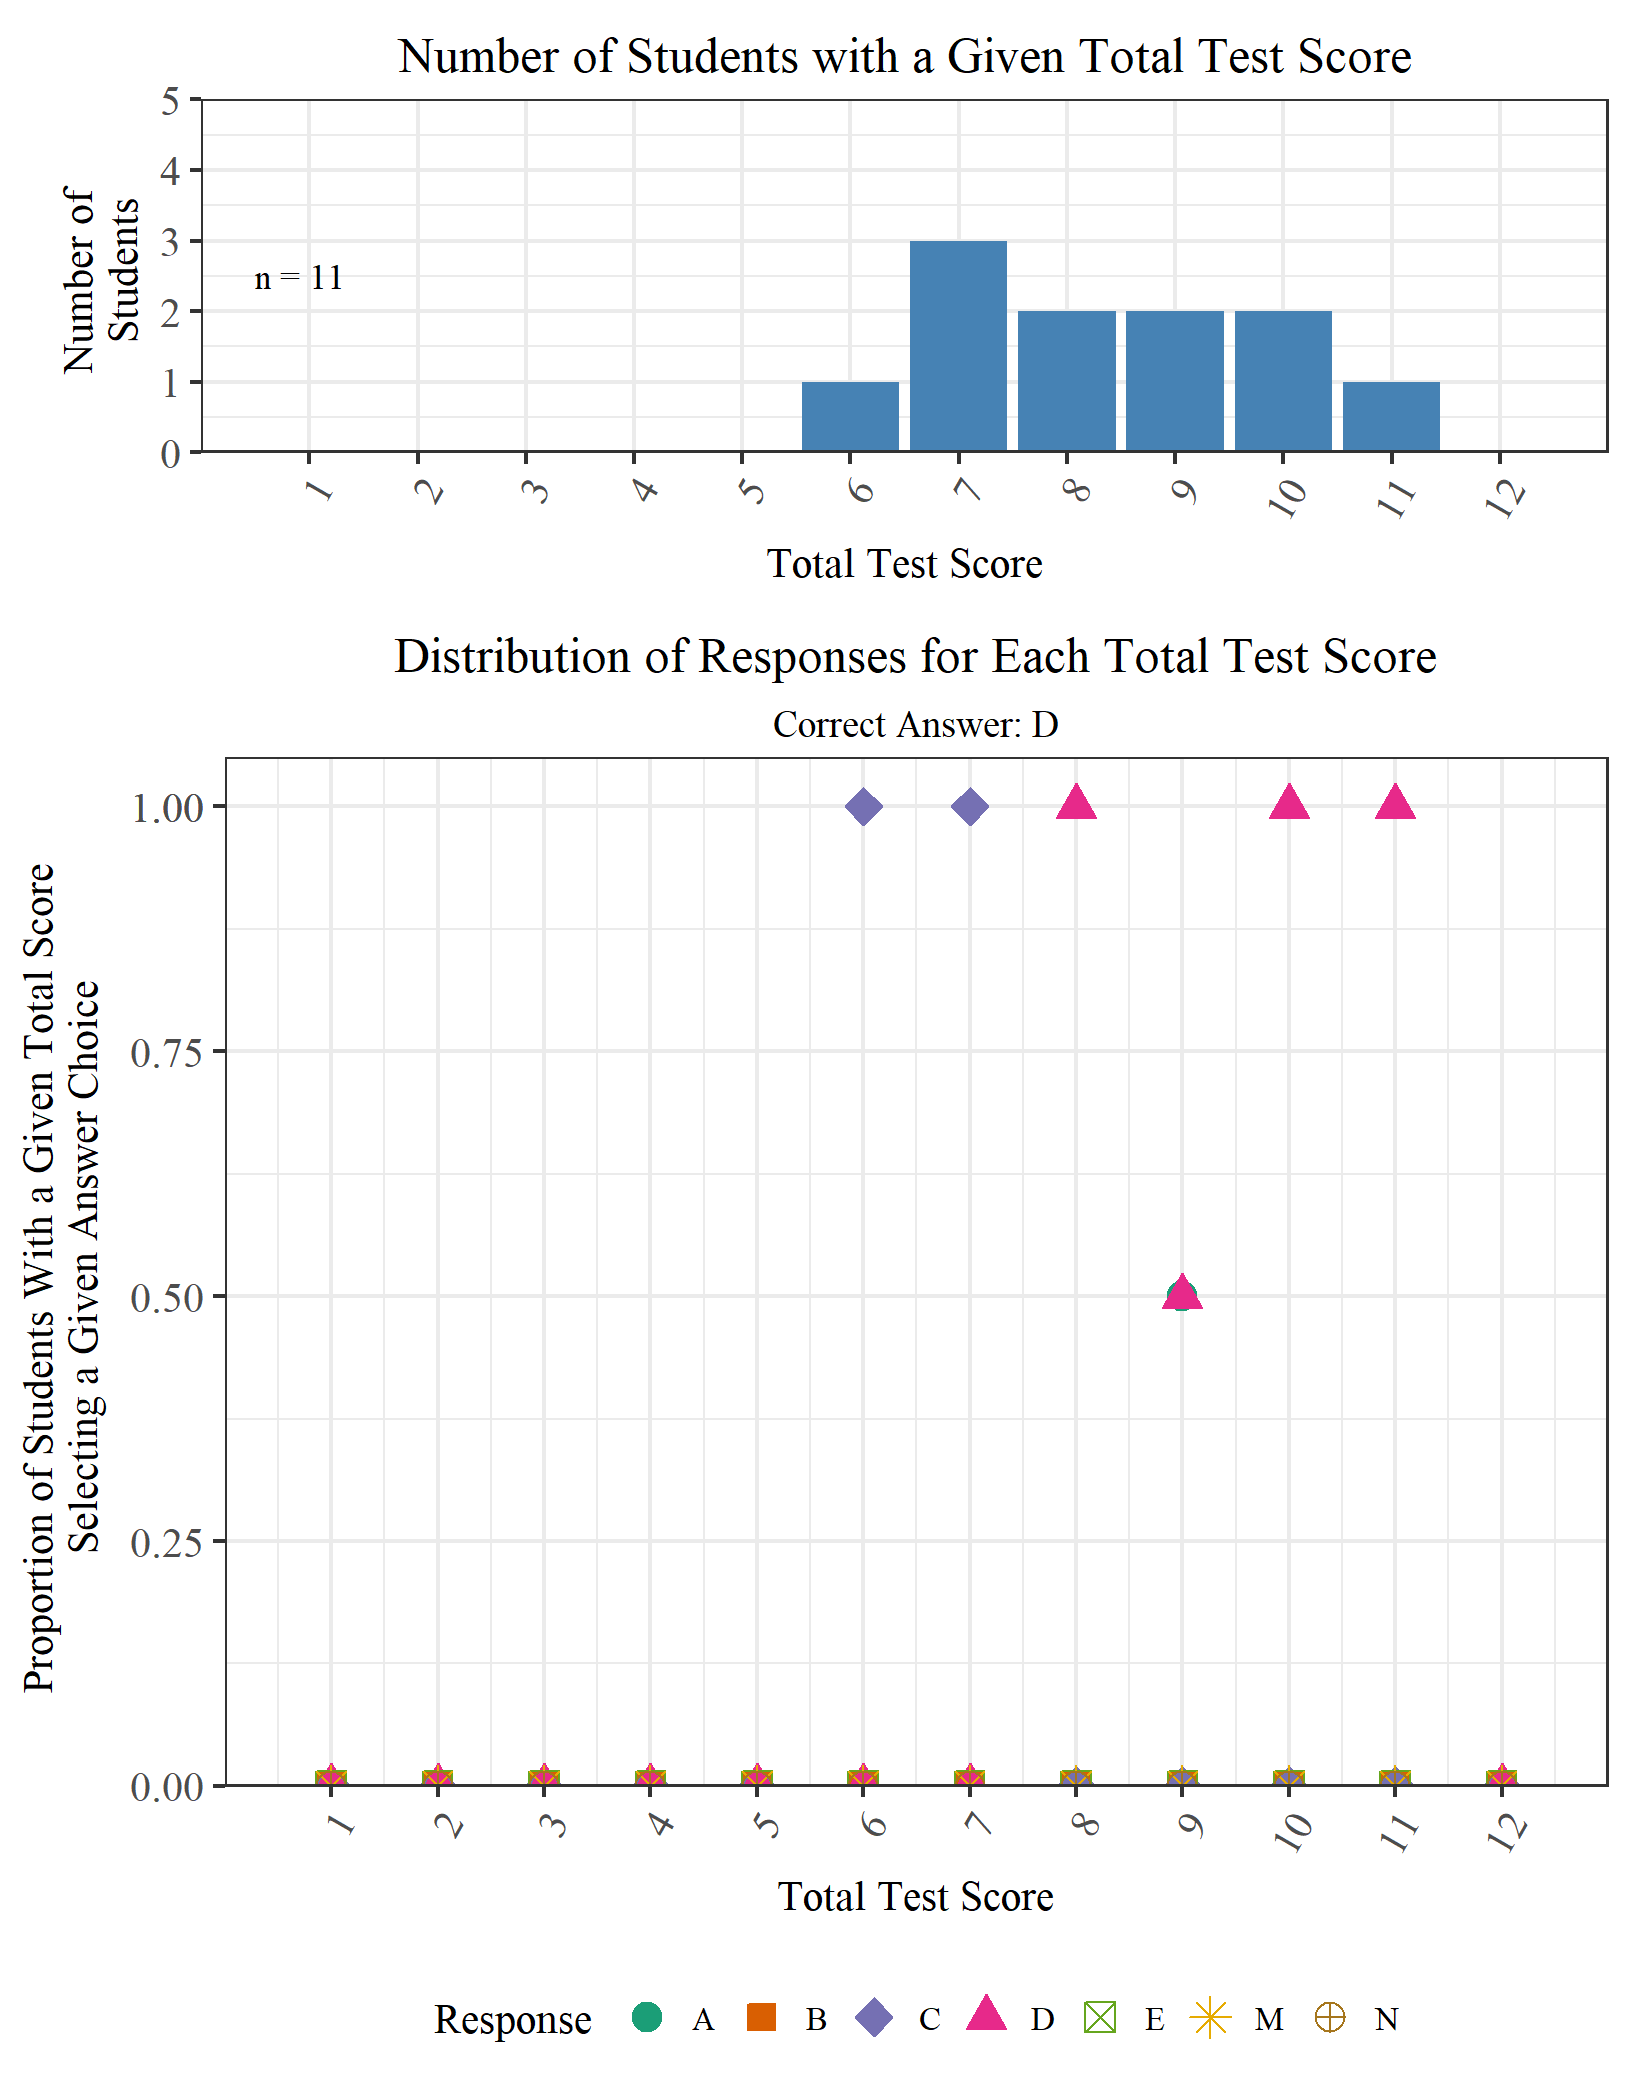
\includegraphics[width=\maxwidth]{IRC_9.png}\newpage\subsection*{Q10. Vector Projection: Coord. System}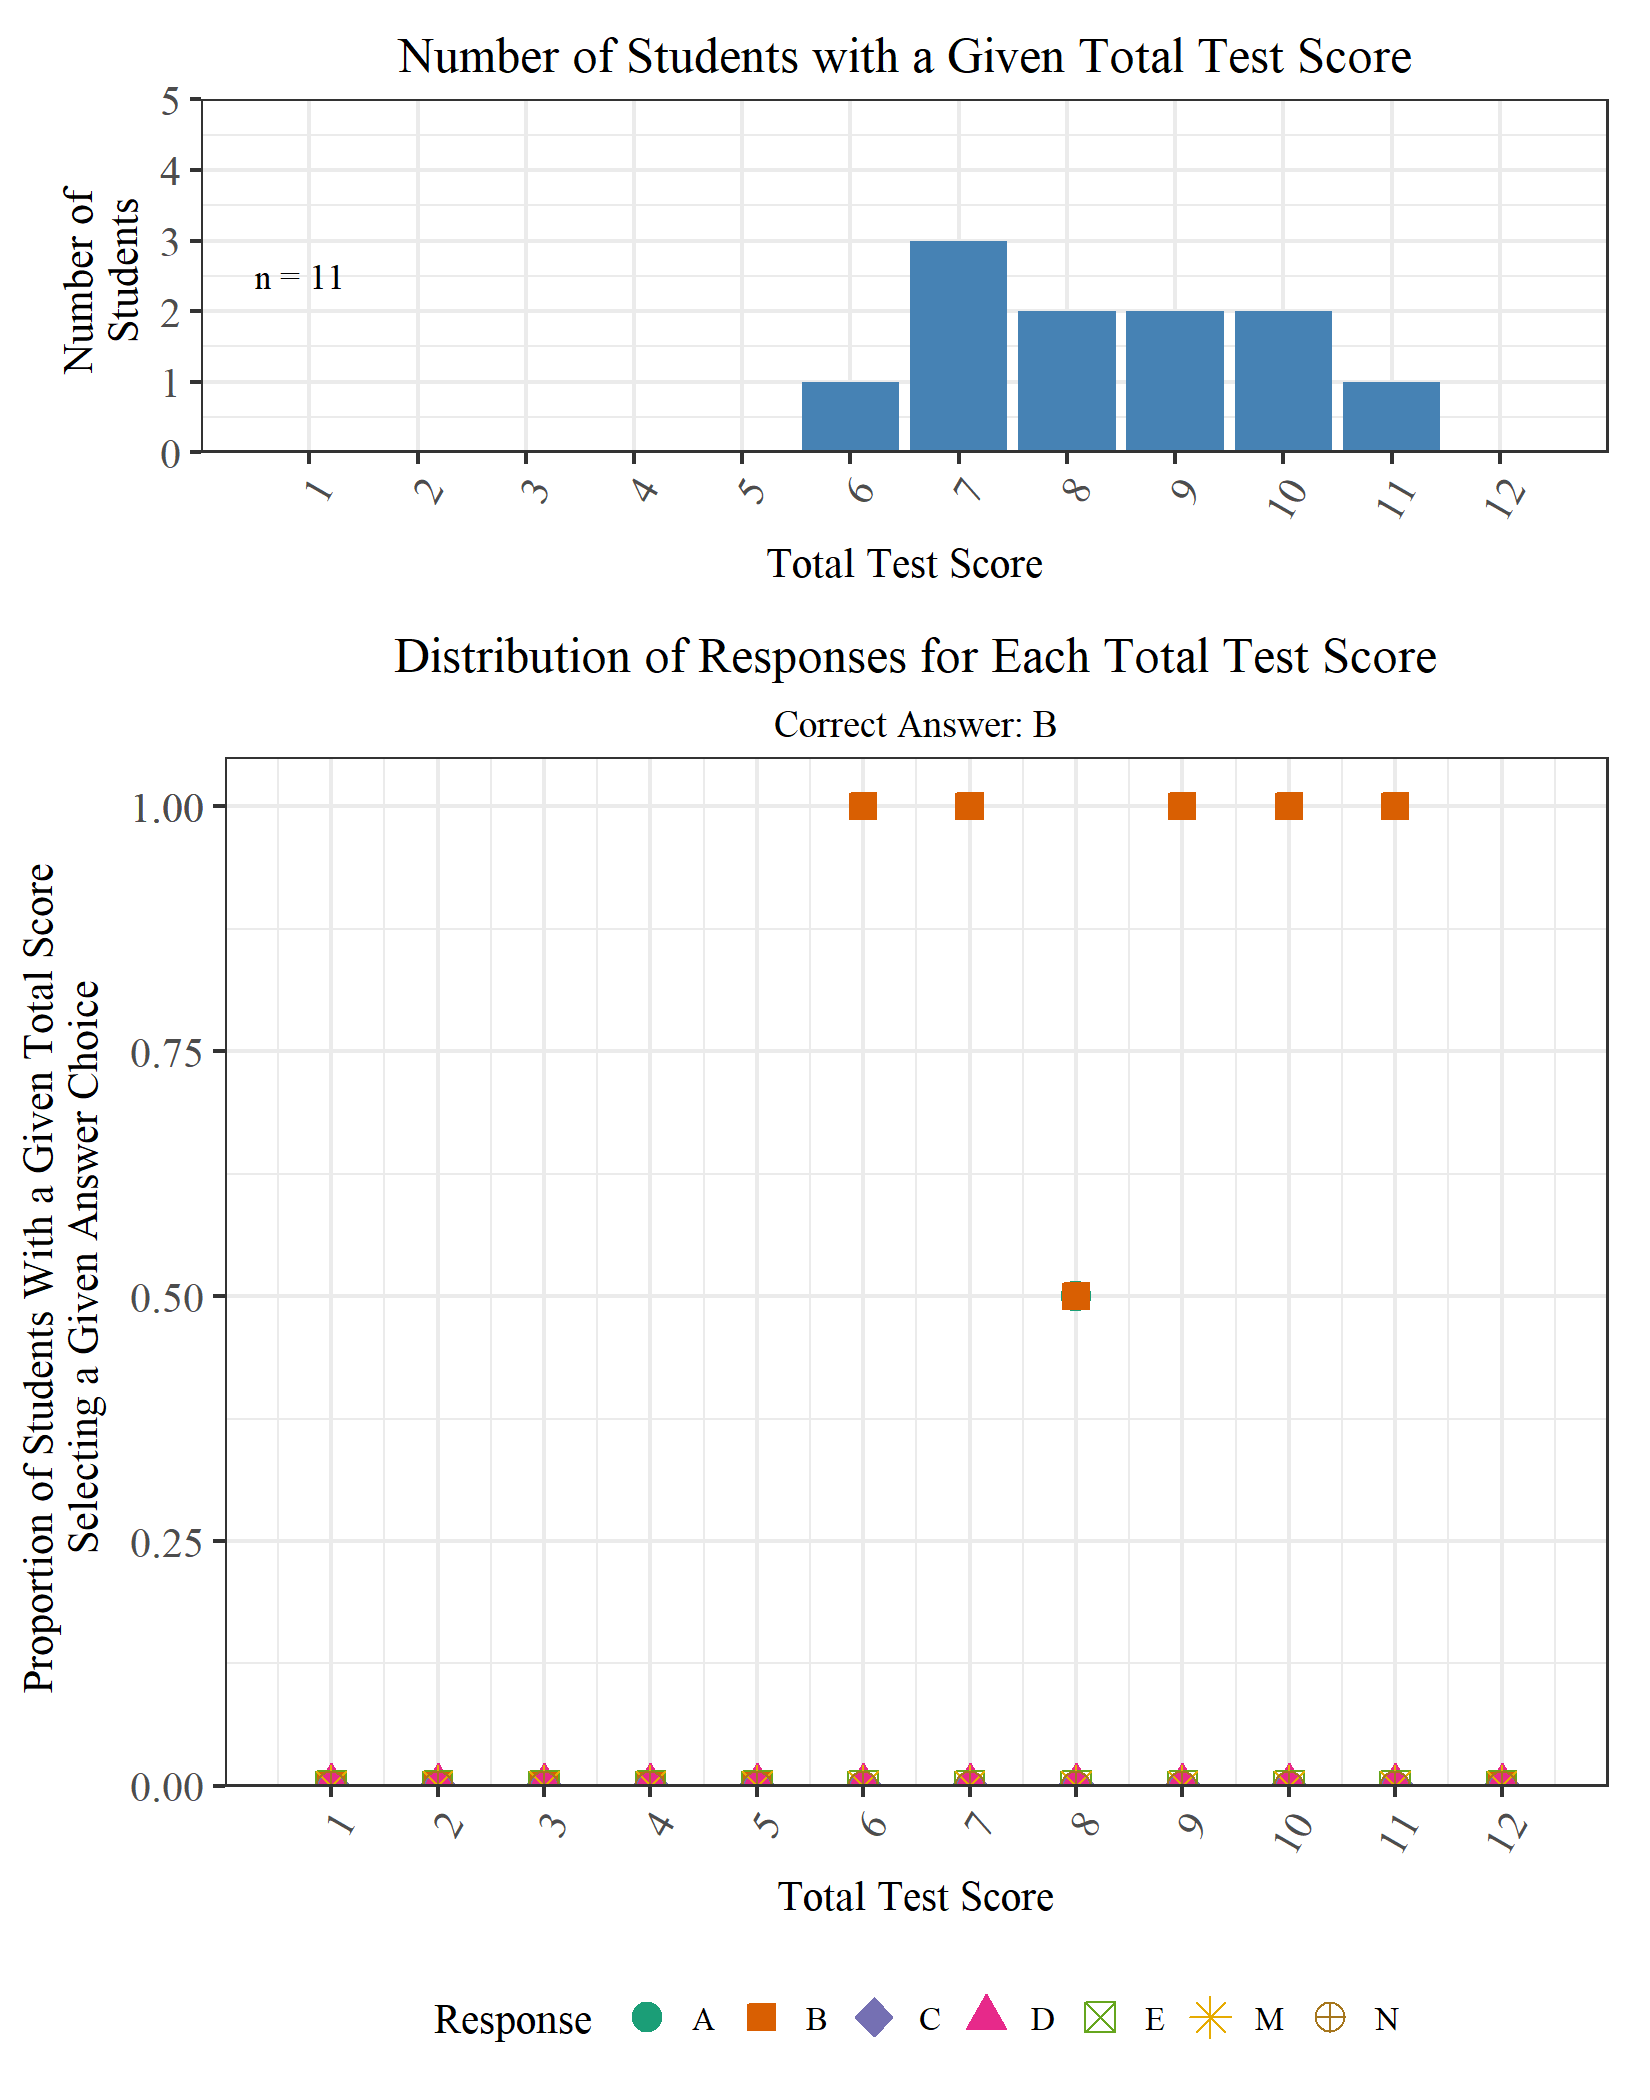
\includegraphics[width=\maxwidth]{IRC_10.png}\newpage\subsection*{Q11. Vector Projection: Rotated Coord. System}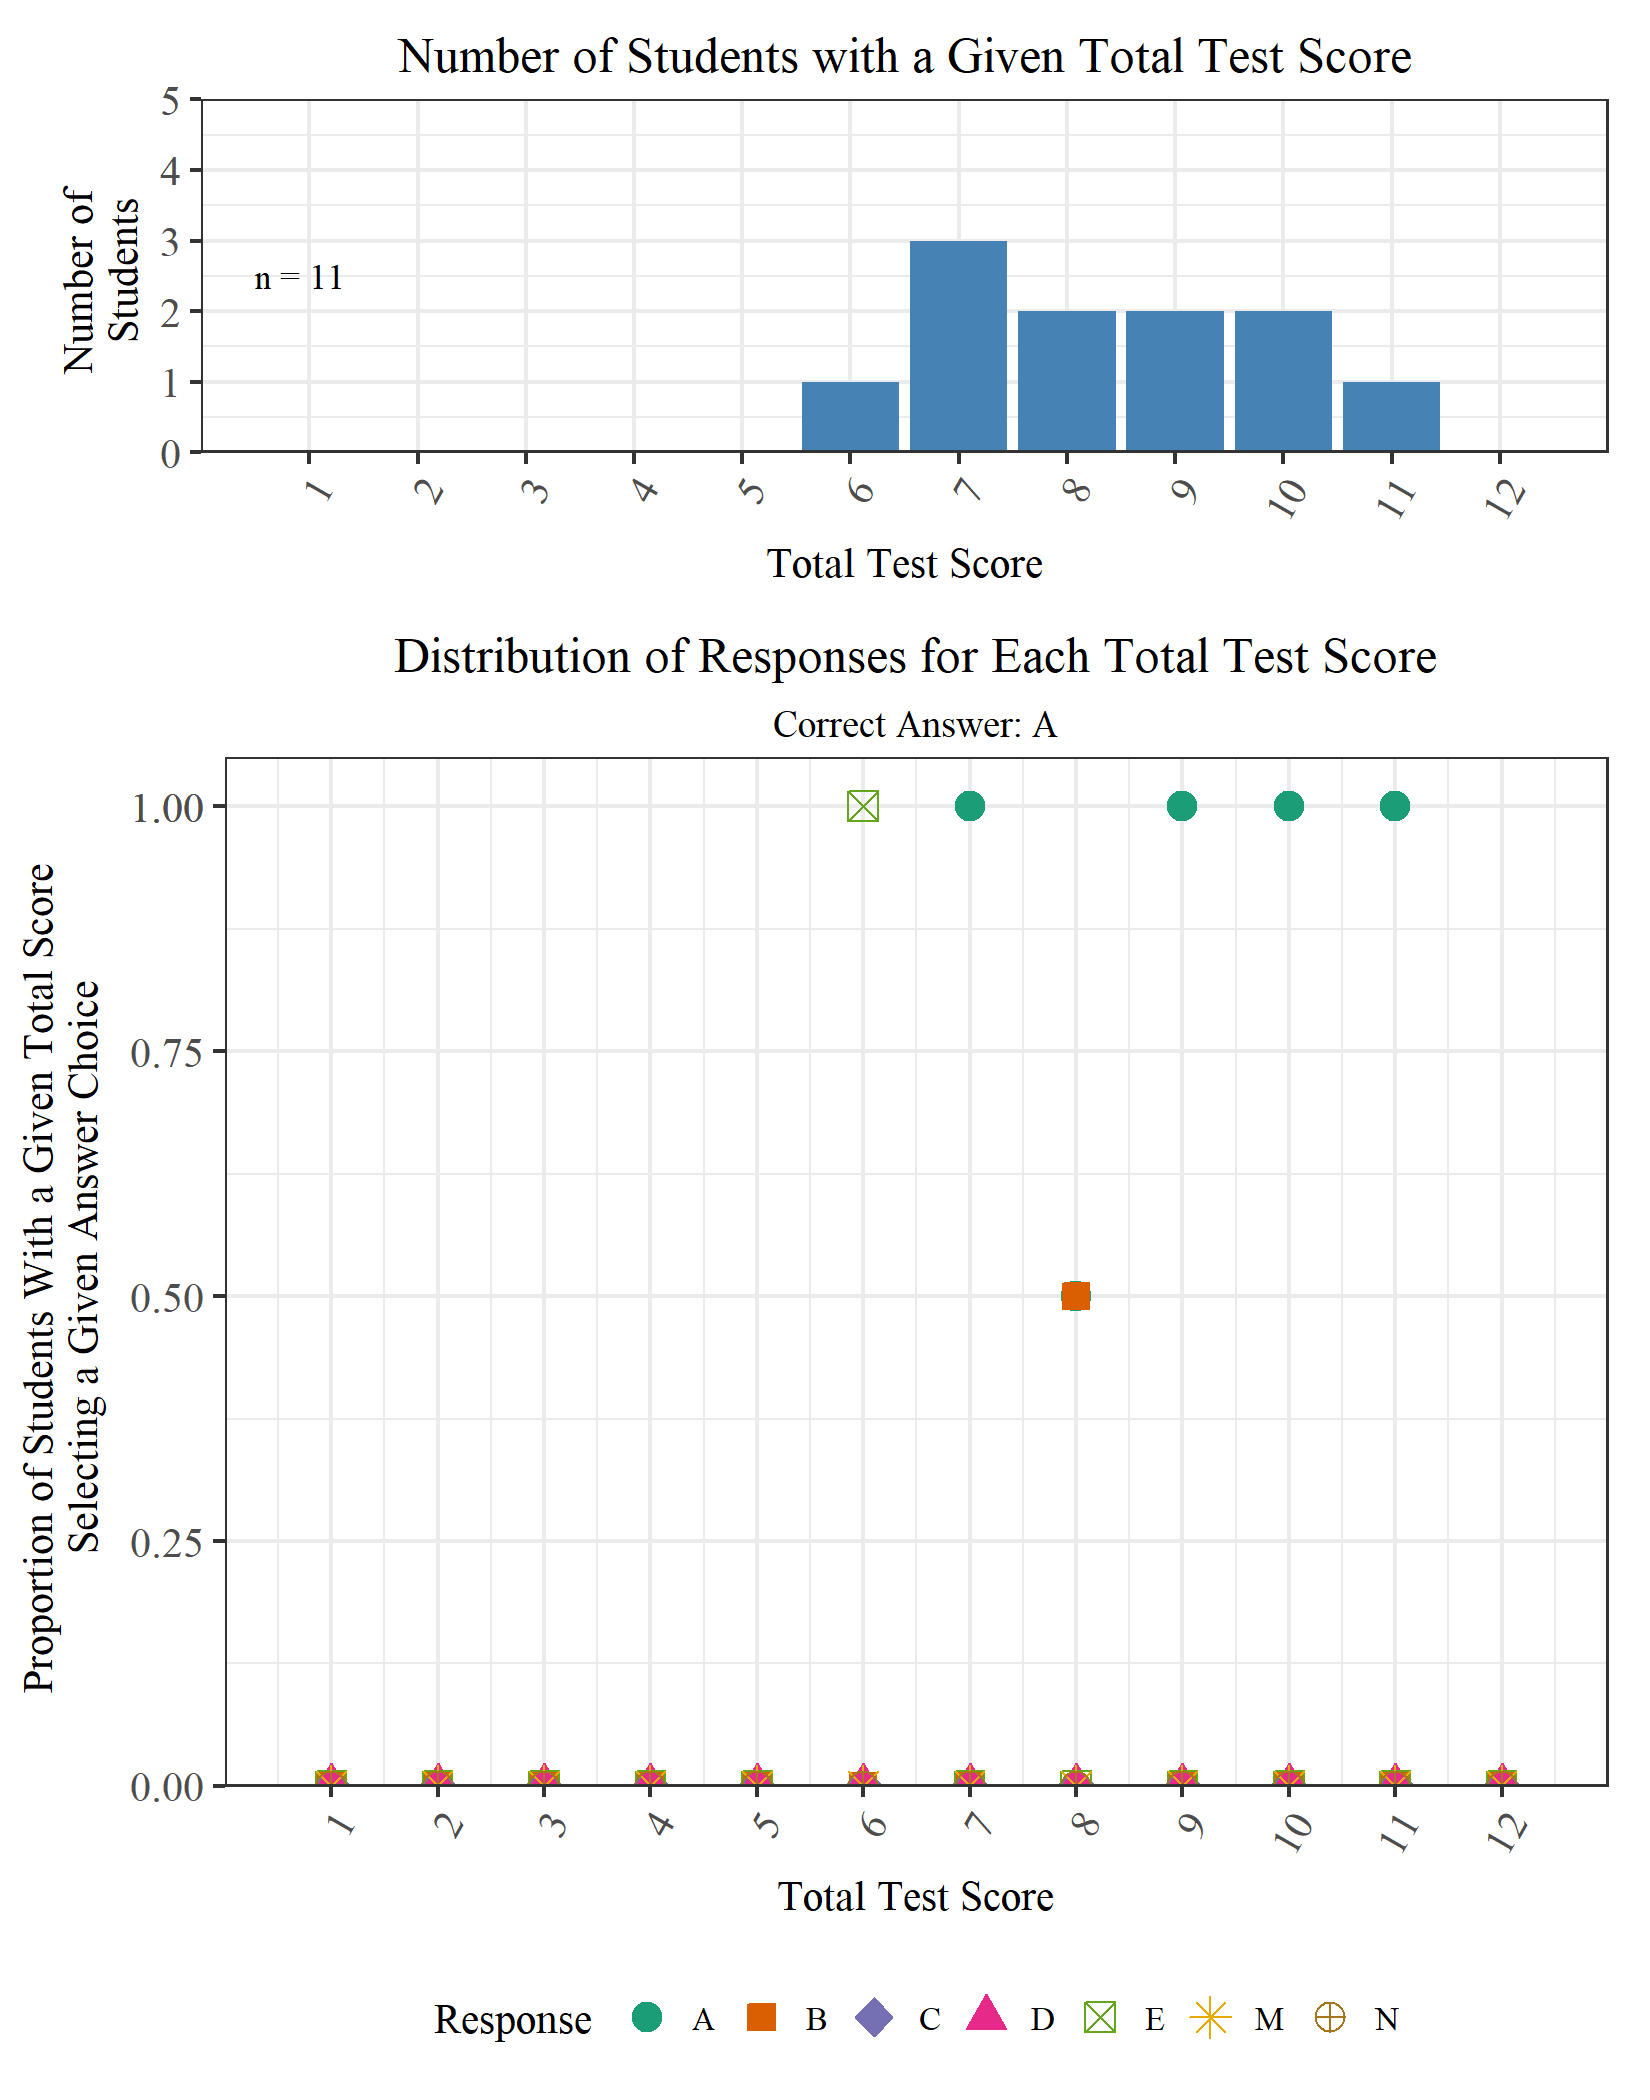
\includegraphics[width=\maxwidth]{IRC_11.png}\newpage\subsection*{Q12. Moments}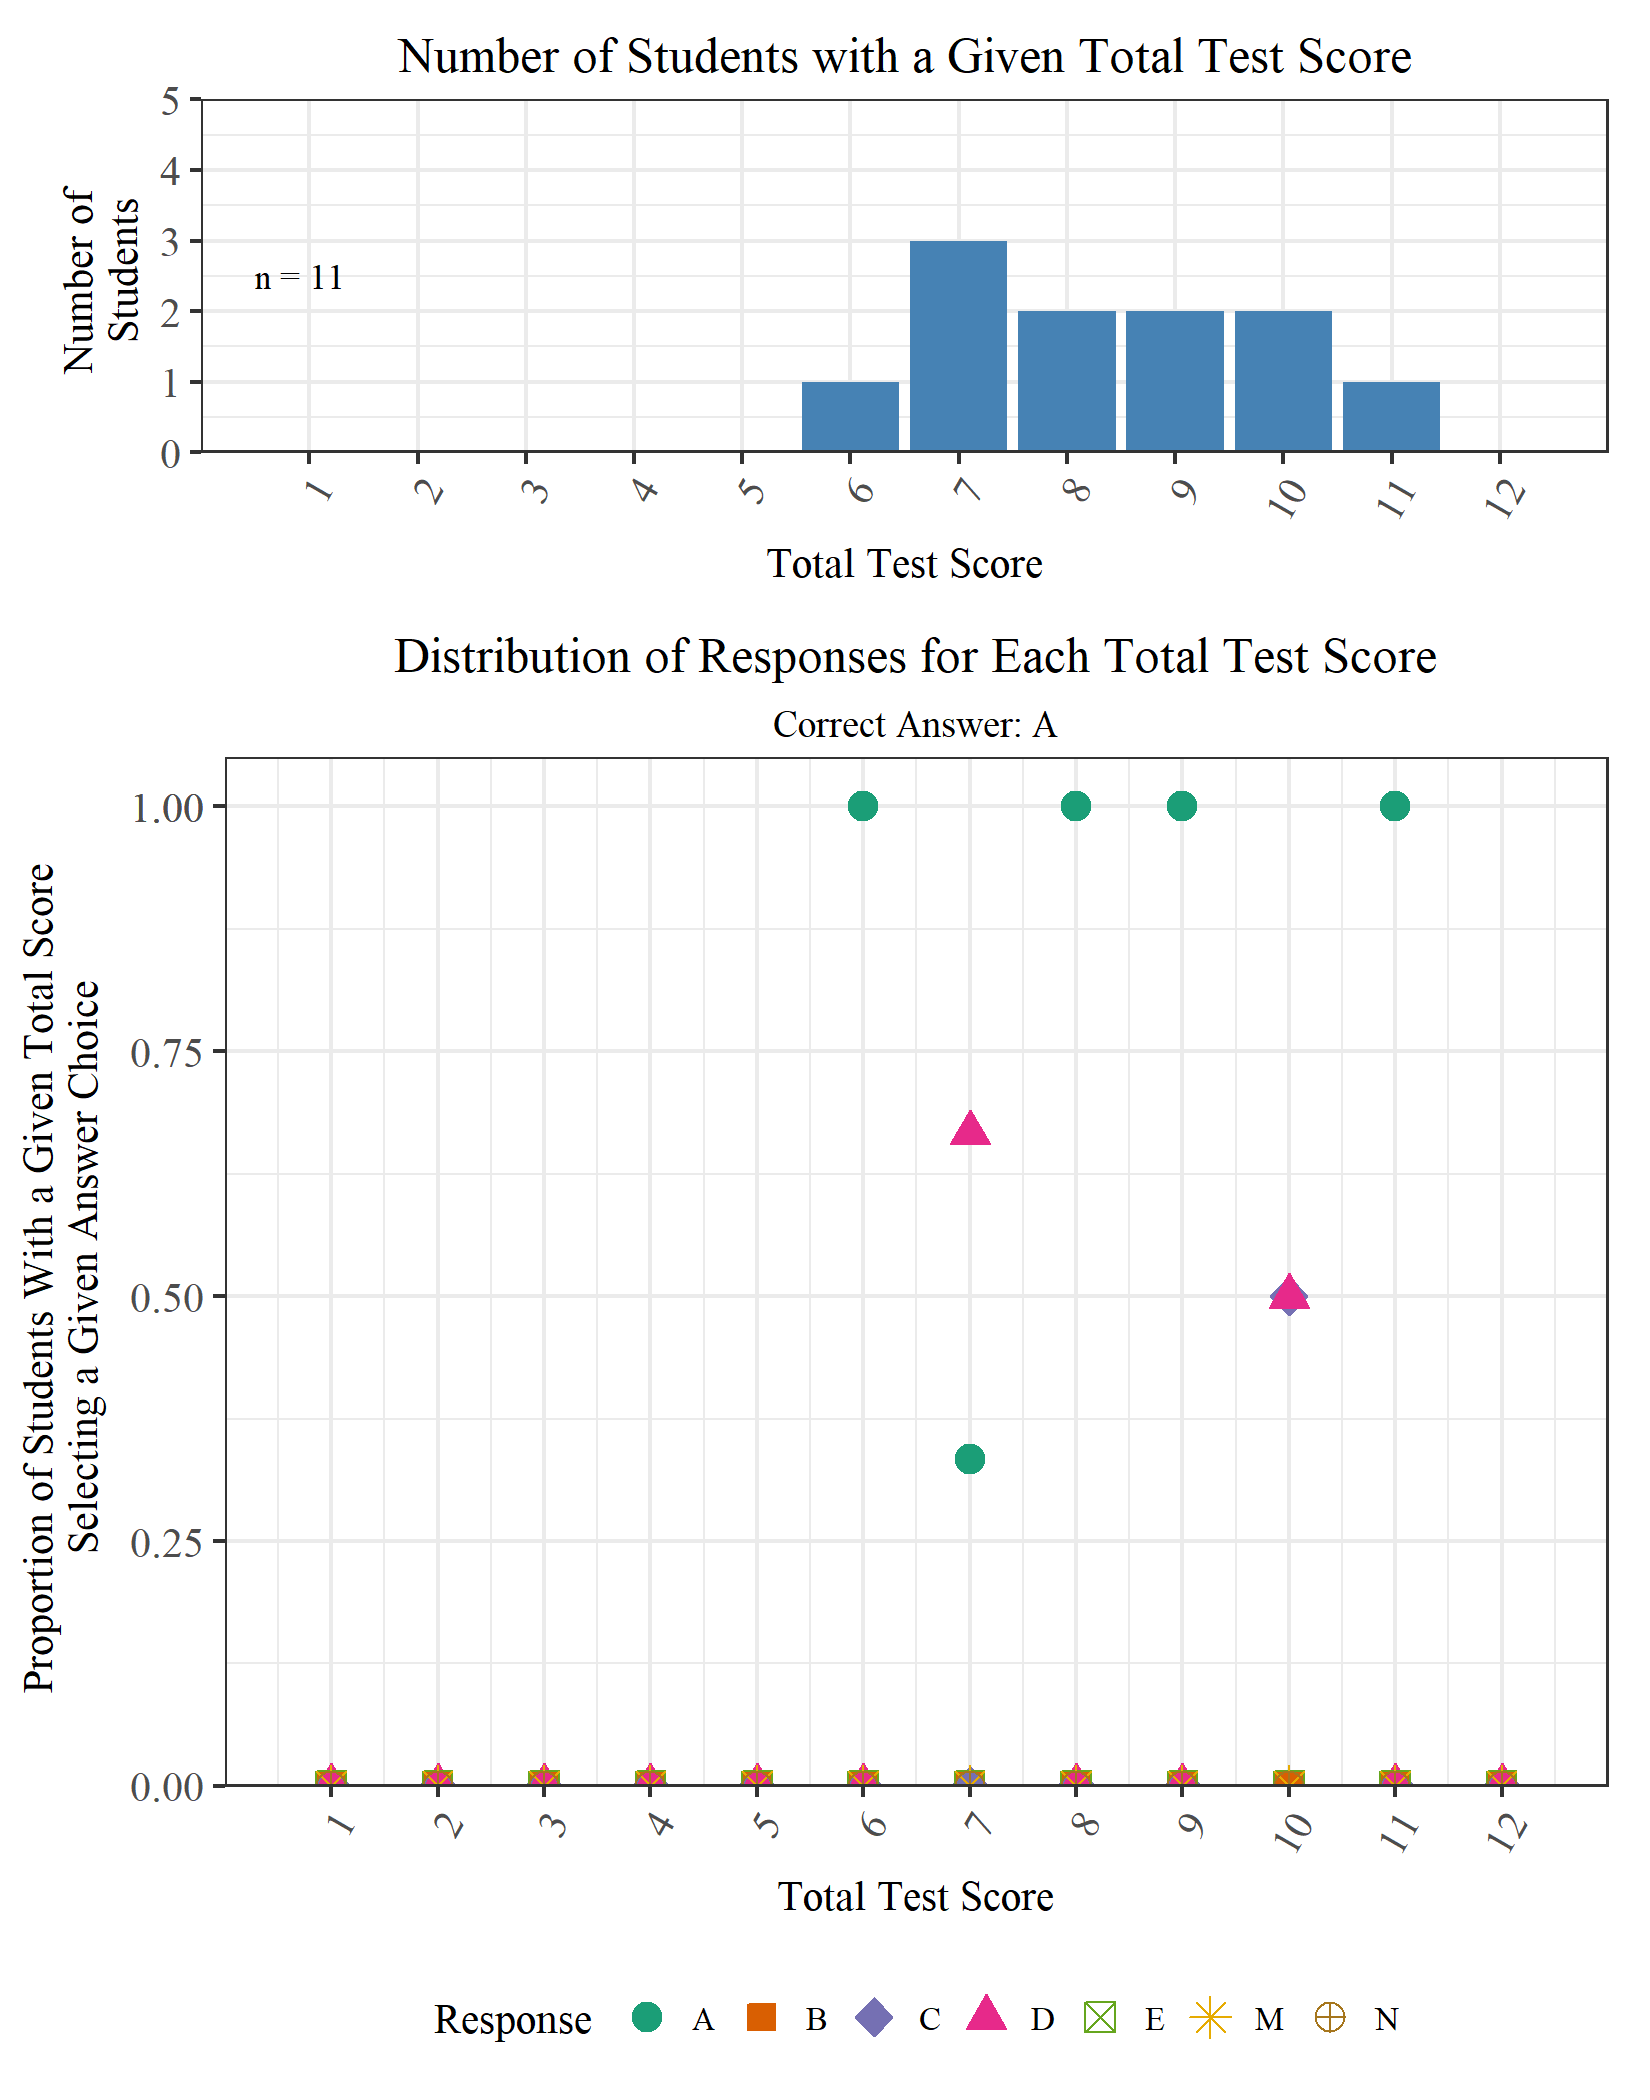
\includegraphics[width=\maxwidth]{IRC_12.png}\newpage


\newpage

\end{document}
